% TODO (master-document merge): this file is compiled standalone as `article`,
% with \section standing in for what will become \chapter once the thesis is
% assembled. Chapter 1 (chapter1_introduction.tex) and Chapter 2
% (chapter2_methodology.tex) are in the same standalone state for the same
% reason. At merge time: switch \documentclass to `report` (or `book`), replace
% this file's top-level \section with \chapter and demote \subsection ->
% \section, \subsubsection -> \subsection accordingly, apply the same demotion
% to every other chapter file, and move all bibliography blocks into a single
% shared bibliography (a .bib file via BibTeX/biblatex, or one merged
% thebibliography) so each chapter stops carrying its own duplicate reference
% list. All \ref/\label numbering (Section 3.1, 3.2, ... and the "Section 1.X" /
% "Section 2.X" cross-references into Chapters 1 and 2 already written
% throughout this file) will resolve automatically to the correct
% chapter-relative numbers once this is done; no cross-reference text needs to
% change by hand.
\documentclass[11pt, a4paper, twoside]{article}

\usepackage[utf8]{inputenc}
\usepackage[a4paper, left=1.5in, right=1.5in, top=1in, bottom=1in]{geometry}
\usepackage{amsmath, amssymb, amsfonts}
\usepackage{textcomp}
\usepackage{booktabs, tabularx, array}
\usepackage{graphicx, caption, subcaption}
\usepackage[hidelinks]{hyperref}
\usepackage{natbib}
\bibliographystyle{plainnat}
\usepackage{newtxtext, newtxmath}
\usepackage{setspace}
\onehalfspacing

% Standalone-build numbering. In the merged thesis this file's top-level
% \section becomes \chapter 3, and LaTeX generates "3.1", "3.1.1", "Table 3.4",
% "Equation (3.7)" automatically. In the standalone build the same objects would
% otherwise be numbered "1", "1.1", "Table 4", "(7)", which collides visually
% with the hardcoded "Section 1.x" / "Section 2.x" / "Table 1.1" / "Table 2.6"
% references into Chapters 1 and 2 that appear throughout this file. The four
% redefinitions below make the standalone build display exactly the numbers the
% merged build will generate, so cross-references read correctly in both.
% DELETE THIS BLOCK at merge time, together with the \documentclass change.
\renewcommand{\thesection}{3.\arabic{section}}
\renewcommand{\thetable}{3.\arabic{table}}
\renewcommand{\thefigure}{3.\arabic{figure}}
\renewcommand{\theequation}{3.\arabic{equation}}

\title{\textbf{Chapter 3 --- Derivatives Pricing, Risk Management and Conclusions}\\[4pt]
\large Continuous-Time Modelling of Wind Speed for Derivatives Pricing and Risk Management}
\author{}
\date{}

\begin{document}

\maketitle

Chapter~2 developed a five-stage modelling pipeline running from raw daily wind speed to a continuous-time stochastic-volatility representation, and reported its fitted parameters for both datasets. This chapter puts those parameters to work. It defines a synthetic variance swap written on German onshore wind generation and prices it on both datasets; it validates the competing forecasting specifications against a persistence benchmark; it quantifies the Value of Information obtained by replacing the geographic proxy with the aligned reference dataset; and it evaluates a Cumulative Accumulated Wind Speed (CAWS) instrument as a left-tail complement to the variance swap. It closes with the thesis's concluding synthesis.

Two conventions carry over from Chapter~2 and govern everything that follows. The first is the benchmark assumption $\theta_1 = \theta_2 = 0$ of Section~2.5.4, adopted because no option-implied data exist for this underlying, under which the physical and pricing measures coincide and the model-implied fair strike reduces to the closed form $K_{\text{var}}^B = h \times C_0$. The second is that all fitted parameters are frozen outputs of the phase notebooks: nothing is re-estimated here. Where a numerical result quoted below differs from the corresponding phase write-up, the executed notebook output is taken as authoritative and the discrepancy is stated rather than reconciled silently, following the practice adopted throughout Chapter~2.\footnote{One naming point is settled here rather than left to the reader. The two Phase~6 source documents are titled ``Phase 6: Carr-Lee Variance Swap Pricing.'' That title misdescribes what those documents implement. \citet{CarrLee2009} is the theoretical motivation for variance-swap replication, reviewed in Section~1.3.6; the formula actually implemented is the closed-form $K_{\text{var}}^B = h \times C_0$ derived under the piecewise-constant-volatility convention of \citet{Tol1997} and the $\theta = 0$ benchmark. No Carr--Lee replication is attempted anywhere in this thesis, and no section of this chapter is named for it.}

\section{The Synthetic Wind Variance Swap}
\label{sec:varswap}

\subsection{Instrument Definition and the Two Tracks}
\label{sec:varswap-def}

A variance swap is a forward contract on realised variance. The long party receives the realised variance of the underlying over the contract period and pays a fixed strike agreed at inception, so that the terminal payoff of a unit-notional position initiated at $t$ and settling at $T$ is
\begin{equation}
\Pi_{[t,T]} = \mathrm{RV}_{[t,T]} - K_{\text{var}}, \qquad
\mathrm{RV}_{[t,T]} = \frac{252}{N_{[t,T]}}\sum_{s=t+1}^{T} r_s^2,
\label{eq:vs-payoff}
\end{equation}
where $r_s$ is the daily log-return of the underlying and $N_{[t,T]}$ the number of returns in the window. The payoff is linear in realised variance: unlike a straddle, there is no gamma scaling and no path-dependent convexity, which is what makes the contract a clean instrument for isolating volumetric volatility risk. A wind producer, whose operating cash flow is naturally long generation volume and therefore short the stability of that volume, takes the opposite side, receiving $K_{\text{var}} - \mathrm{RV}_{[t,T]}$.

The underlying chosen here is not wind speed but German onshore wind generation, the SMARD aggregate documented in Section~1.4.3. This choice is deliberate: it is generation, not wind speed at a point, that determines a producer's revenue, and it is generation for which a market-observable series exists over the full ten-year window. The wind-speed model of Chapter~2 enters through the power-curve linkage $G \propto W^3$ developed in Section~\ref{sec:powercurve}.

Two fair strikes are computed, and the distinction between them organises the whole of this section.

\begin{description}
\item[Track A (empirical).] $K_{\text{var}}^A(t) = 252 \times \overline{\mathrm{RV}}_t^{(252)}$, the $252\times$-annualised rolling mean of the daily realised variance $\mathrm{RV}_t = r_t^2$ of SMARD generation log-returns. This is a purely empirical quantity requiring no model: it is what the market data themselves say a fair strike would have been.
\item[Track B (model-implied).] $K_{\text{var}}^B(h) = h \times C_0$, the closed-form strike implied by the CAR(4)+GARCH model under the piecewise-constant-$h$ convention of \citet{Tol1997}, in which $h$ is frozen at its pricing-date value over the life of the contract and the first and second Fourier harmonics of $\sigma^2_{\text{seasonal}}(t)$ integrate to zero over a full contract year, leaving only the constant $C_0$ (Section~2.3.2).
\end{description}

These two quantities measure the variance of different processes, expressed in different units and under different annualisation conventions. Their raw numerical gap, between two and three orders of magnitude (a factor of about $130$ for Dataset~B and $2{,}100$ for Dataset~A), is therefore not a measure of model error, and no comparison between them is drawn in this chapter before the reconciliation of Section~\ref{sec:reconciliation}. This point was flagged in Section~1.5 and is developed quantitatively below; it is the single most consequential piece of bookkeeping in the chapter.

\subsection{Market Data: Generation and Day-Ahead Prices}
\label{sec:market-data}

The SMARD files described in Section~1.4.3 yield 87{,}662 hourly observations spanning 1~January~2015 to 31~December~2024. Aggregating generation as the sum of the 24 hourly values within each day gives 3{,}653 daily observations with no missing values, no day exceeding the 20\% missing-hour threshold, and no day recording zero aggregate generation; the two filters described in Section~1.4.3 therefore removed nothing. Mean daily generation is 255{,}560~MWh with a standard deviation of 196{,}107~MWh, and the series ranges from 7{,}214~MWh on the calmest day of the decade to 1{,}060{,}474~MWh on the windiest. That the standard deviation is roughly three-quarters of the mean, and that the maximum exceeds the minimum by a factor of 147, is the basic fact that motivates a volumetric hedge at all.

The day-ahead price series, merged across the October~2018 bidding-zone split as specified in Section~1.4.3, is four days shorter: the SMARD price files carry no quotation for 1--4~January~2015, so the aligned generation-and-price sample runs from 5~January~2015 and contains 3{,}649 days. Mean price over the full sample is \texteuro{}71.38/MWh with a standard deviation of \texteuro{}78.05/MWh, and the range runs from $-$\texteuro{}53.87/MWh to \texteuro{}699.44/MWh. The negative minimum is not a data error: it is the well-documented consequence of inflexible must-run capacity meeting high renewable infeed at low demand, and it is precisely the state of the world the merit-order analysis of Section~\ref{sec:merit} examines.

This four-day difference between the generation sample (3{,}653 days) and the aligned sample (3{,}649 days) is the sole reason the two Track~A strikes reported below differ, and it is recorded here so that the discrepancy is not mistaken for a substantive one.

\begin{figure}[htbp]
\centering
\begin{subfigure}{0.9\textwidth}
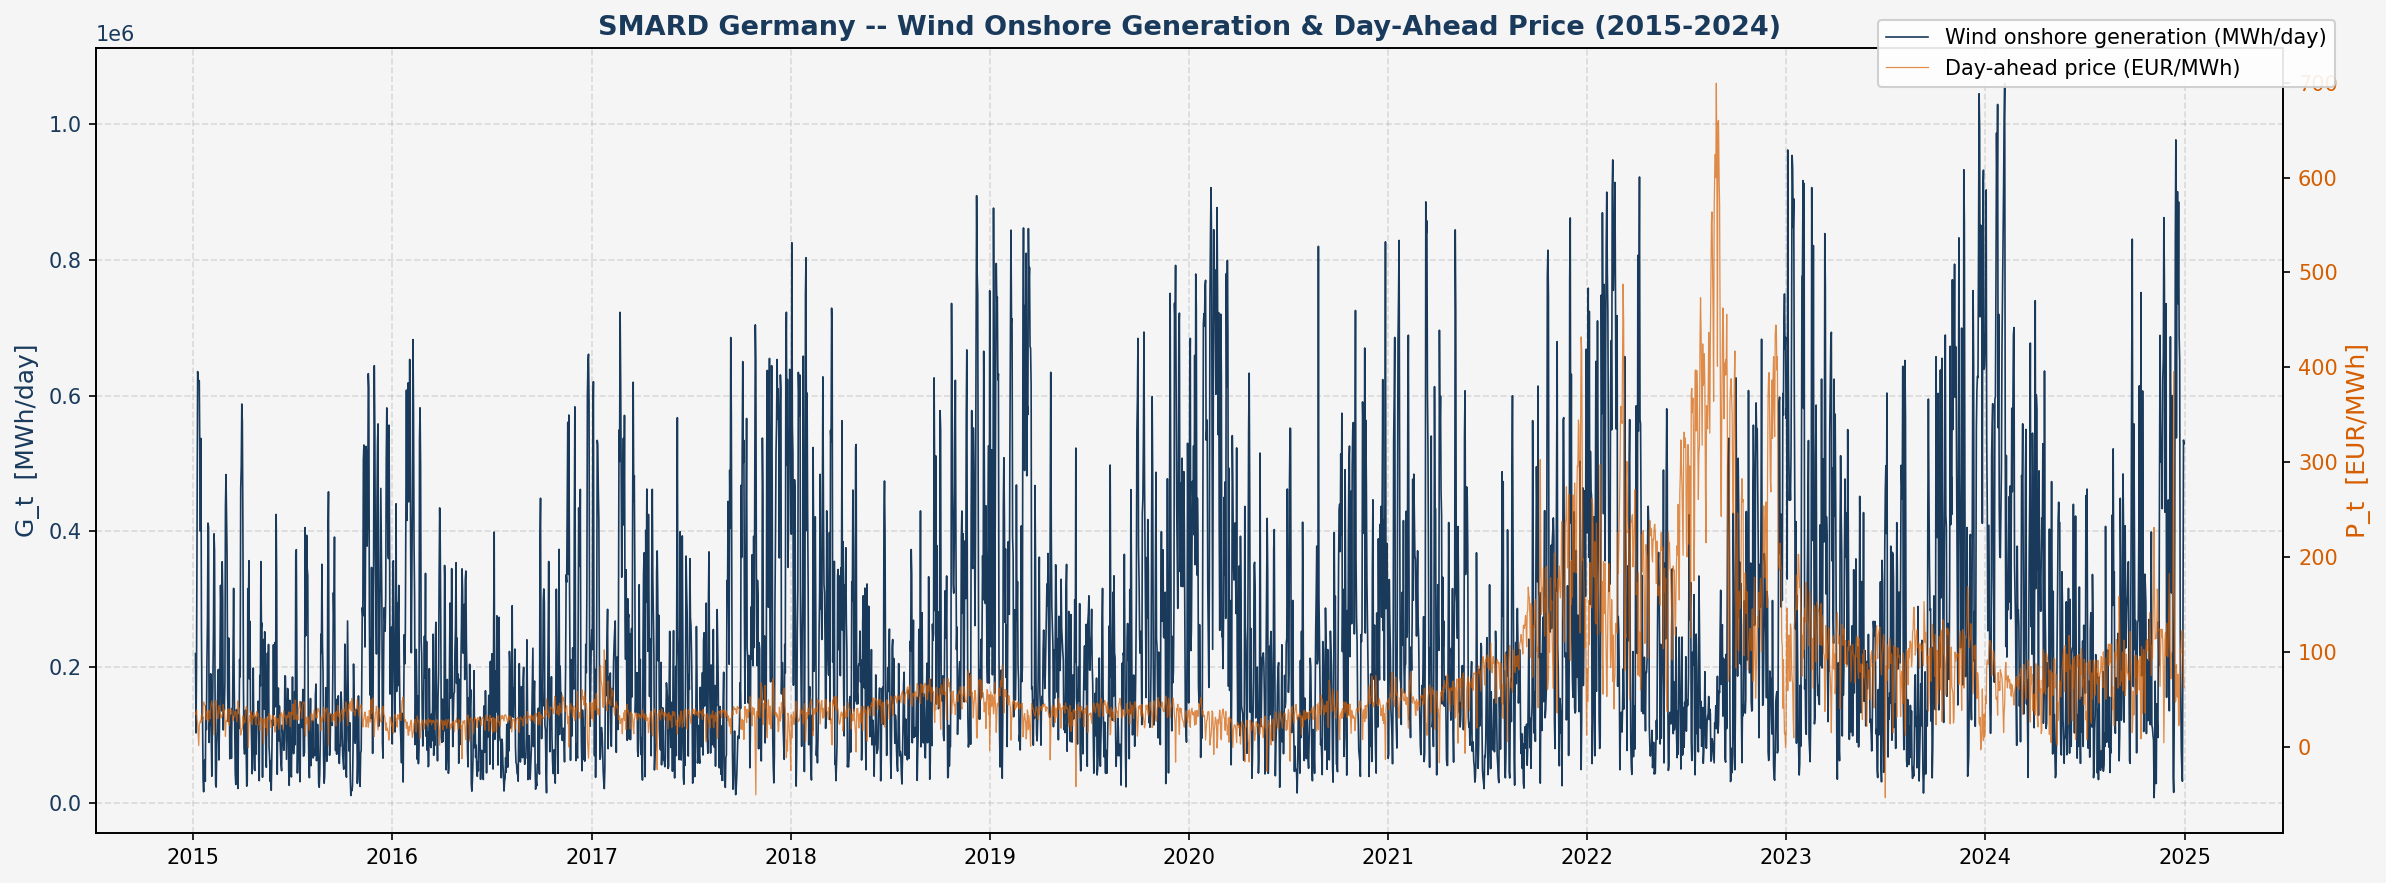
\includegraphics[width=\textwidth]{figures/phase6_B_smard_overview.png}
\caption{SMARD daily generation and day-ahead price}
\end{subfigure}
\\[6pt]
\begin{subfigure}{0.9\textwidth}
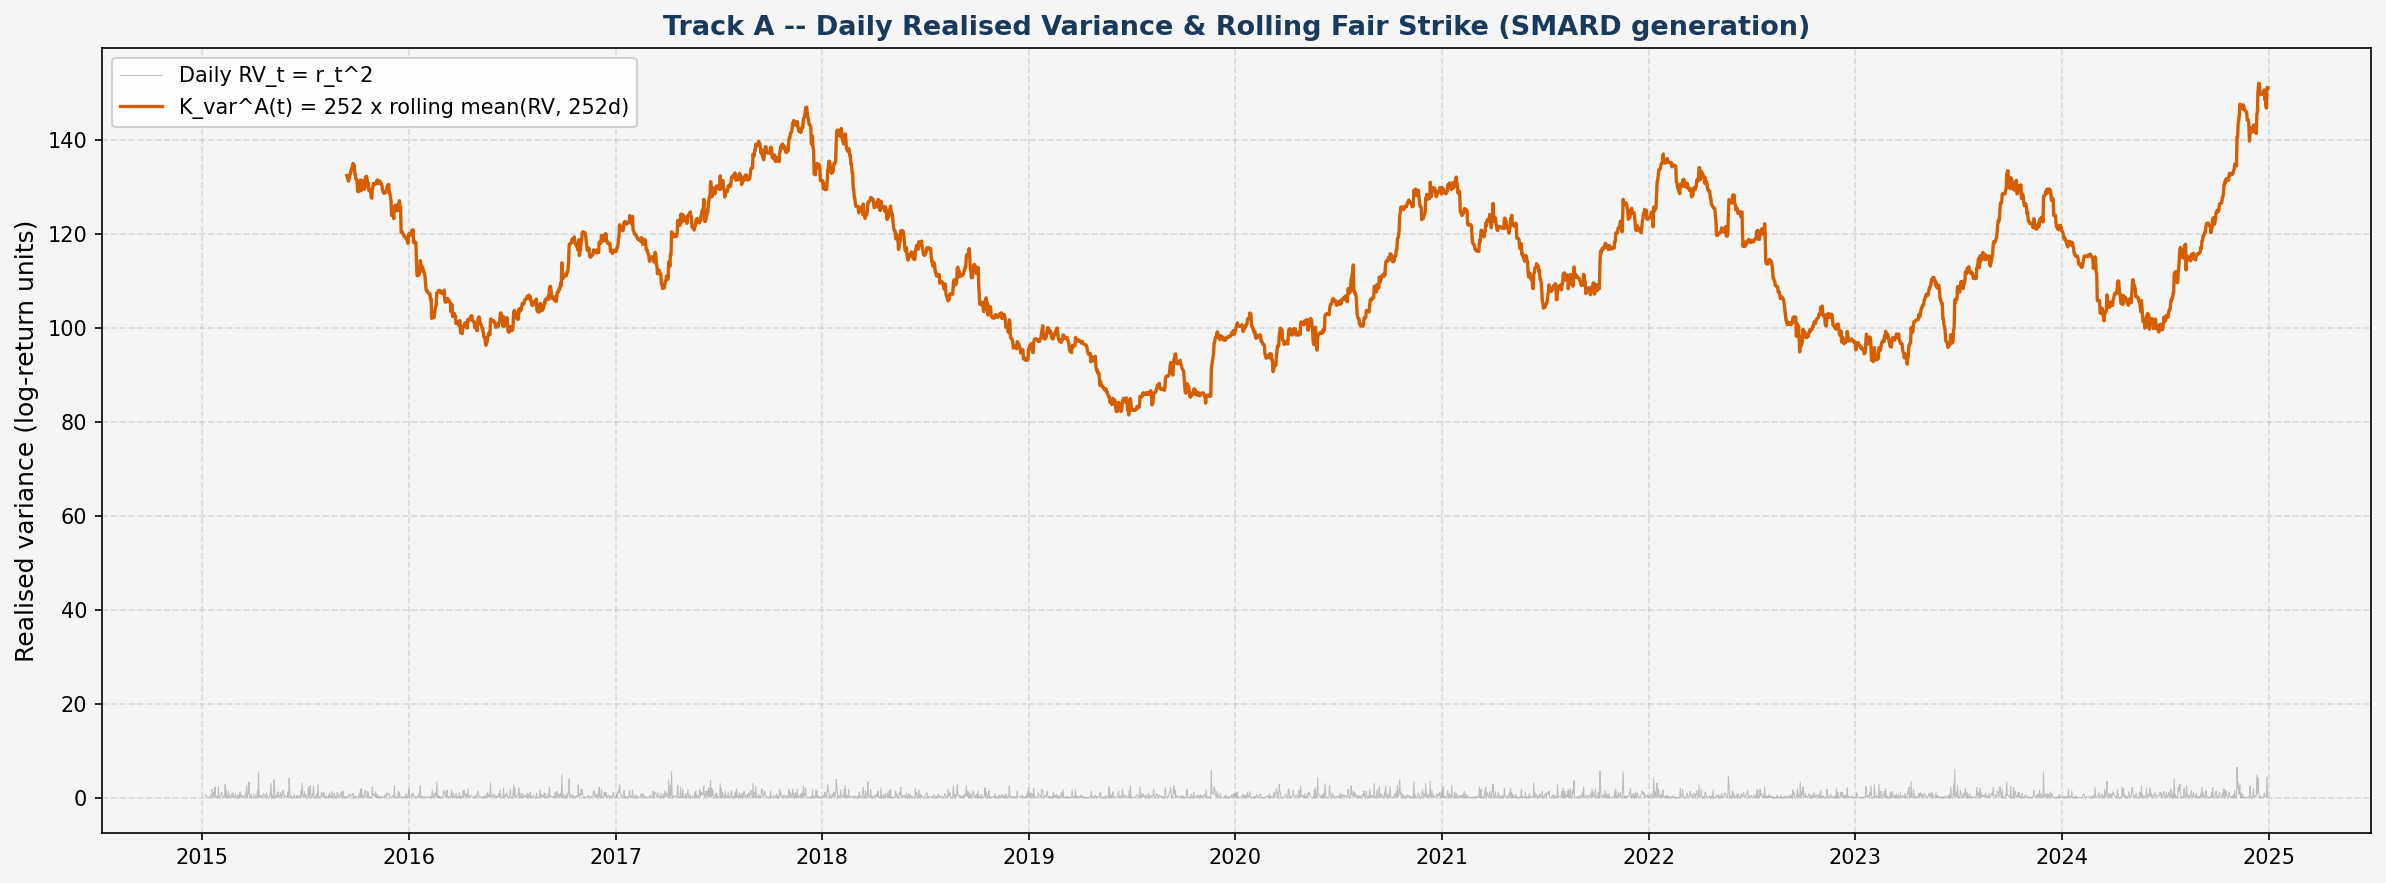
\includegraphics[width=\textwidth]{figures/phase6_B_rv_tracka.png}
\caption{Track A: daily realised variance and rolling fair strike}
\end{subfigure}
\caption{Market data and the empirical fair strike. \textbf{(a)} Daily German onshore wind generation $G_t$ in MWh/day (left axis) and the merged day-ahead price $P_t$ in \texteuro{}/MWh (right axis), 2015--2024, on a dual-axis plot. The price series' change of level from 2021 onward is the European energy-price crisis discussed in Section~1.4.3, not a change in the generation series. \textbf{(b)} The daily realised variance $\mathrm{RV}_t = r_t^2$ of generation log-returns (thin grey) with the $252$-day rolling annualised fair strike $K_{\text{var}}^A(t)$ overlaid (heavy line). Because the market data are common to both datasets, these two panels are identical up to the four-day alignment difference of Section~\ref{sec:market-data} and are shown once rather than as a dataset pair.}
\label{fig:market-data}
\end{figure}

\subsection{Track A: The Empirical Fair Strike}
\label{sec:tracka}

Log-returns are computed as $r_t = \log(G_t/G_{t-1})$ and set to missing whenever either $G_t$ or $G_{t-1}$ is zero or absent. On the 3{,}653-day generation sample this leaves 3{,}652 valid returns and a mean daily realised variance of $\overline{\mathrm{RV}} = 0.4580$; on the 3{,}649-day price-aligned sample it leaves 3{,}648 returns and $\overline{\mathrm{RV}} = 0.4583$. The corresponding full-sample means of the rolling annualised strike are
\begin{equation}
K_{\text{var}}^A = 113.999 \ \text{(generation sample)}, \qquad
K_{\text{var}}^A = 113.145 \ \text{(price-aligned sample)},
\end{equation}
a difference of 0.75\% arising entirely from the four missing January~2015 price days and the consequent shift in the rolling window's start date. Both figures are reported because the Dataset~A and Dataset~B pricing exercises were run on the two respective samples, and the difference propagates into every Track~A quantity below. It carries no substantive content: Track~A is a property of the German electricity market, not of either wind dataset, and it is identical across the two analyses up to this alignment.

A strike of 114 is very large by the standards of financial variance swaps, where equity-index strikes typically sit in the range 10--25. It corresponds to an annualised volatility of $\sqrt{114} \approx 10.7$, that is, a daily standard deviation of generation log-returns of about 67\%. This is not an artefact: German aggregate wind output routinely changes by a factor of two or more from one day to the next as frontal systems cross the country, and the log-return of such a change is of order $\pm 0.7$. The magnitude is a statement about the underlying, not about the estimator.

\begin{table}[htbp]
\centering
\caption{Track A: seasonal realised variance of SMARD generation log-returns, annualised.}
\label{tab:tracka-seasonal}
\begin{tabular}{l r r}
\toprule
\textbf{Season} & \textbf{Dataset A sample} & \textbf{Dataset B sample} \\
\midrule
DJF (winter) & $100.76$ & $100.99$ \\
MAM (spring) & $115.38$ & $115.38$ \\
JJA (summer) & $119.32$ & $119.32$ \\
SON (autumn) & $126.01$ & $126.01$ \\
\midrule
Full sample $K_{\text{var}}^A$ & $113.999$ & $113.145$ \\
\bottomrule
\end{tabular}
\par\vspace{4pt}
\begin{minipage}{0.92\textwidth}
\footnotesize The two columns are the same market series computed on the two samples of Section~\ref{sec:market-data}; only the winter figure is affected by the four-day alignment, because the missing days fall in January. Dataset~B's source analysis reports these as daily means (DJF $0.4008$, MAM $0.4579$, JJA $0.4735$, SON $0.5000$); they are annualised here by the factor 252 to match Dataset~A's convention.
\end{minipage}
\end{table}

Table~\ref{tab:tracka-seasonal} reports the seasonal decomposition, and its pattern requires comment because it runs opposite to the one established for wind speed in Chapter~2. Section~2.1.3 found the seasonal variance of wind \emph{speed} to peak in winter in both datasets, by a ratio of roughly $6.9{:}1$ for Dataset~A and $1.55{:}1$ for Dataset~B. The realised variance of generation \emph{log-returns} does the reverse: winter is the calmest season on this measure (100.8) and autumn the most volatile (126.0), with summer (119.3) also above winter.

The reversal is a consequence of the log transformation rather than a contradiction. A log-return measures relative change. In winter, generation is high, so a given absolute swing in MWh is a small proportional move; in summer, when mean output is low, the same absolute swing is a large proportional one. Because the seasonal cycle in the \emph{level} of generation is stronger than the seasonal cycle in its absolute variability, the ratio inverts. This matters for a practical reason and is worth stating plainly: a seasonal variance swap on generation log-returns would be priced highest for a summer or autumn contract, exactly opposite to the intuition a producer would form from the seasonal wind-speed cycle. Both Phase~6 source documents assert the opposite pattern, reporting a winter figure of 144 against a summer figure of 80; neither figure appears in either notebook's executed output, and Table~\ref{tab:tracka-seasonal} reports the computed values.

\subsection{Track B: The Model-Implied Fair Strike}
\label{sec:trackb}

Track~B is evaluated at four values of the conditional-variance state $h$, following the scenario design specified for both datasets: the end-of-sample value $h(t_0)$, the winter (DJF) and summer (JJA) means of the fitted $h(t)$ series, and the Gaussian baseline $h = 1$, at which the GARCH layer is switched off and the strike reduces to the pure Fourier seasonal constant. Table~\ref{tab:trackb} reports the resulting strikes for both datasets.

\begin{table}[htbp]
\centering
\small
\caption{Track B: model-implied fair strike $K_{\text{var}}^B(h) = h \times C_0$, four scenarios, both datasets.}
\label{tab:trackb}
\begin{tabular}{l r r r r}
\toprule
& \multicolumn{2}{c}{\textbf{Dataset A} ($C_0 = 0.13138$)} & \multicolumn{2}{c}{\textbf{Dataset B} ($C_0 = 1.16277$)} \\
\textbf{Scenario} & \textbf{$h$} & \textbf{$K_{\text{var}}^B$} & \textbf{$h$} & \textbf{$K_{\text{var}}^B$} \\
\midrule
$h(t_0)$, end of sample & $0.4137$ & $0.05435$ & $0.7511$ & $0.87336$ \\
$h_{\text{winter}}$ (DJF mean) & $0.5559$ & $0.07304$ & $0.7384$ & $0.85861$ \\
$h_{\text{summer}}$ (JJA mean) & $0.6877$ & $0.09036$ & $0.7660$ & $0.89069$ \\
$h = 1$ (Gaussian baseline) & $1.0000$ & $0.13138$ & $1.0000$ & $1.16277$ \\
\bottomrule
\end{tabular}
\end{table}

Three features of the table deserve comment.

First, in both datasets the summer scenario produces a \emph{higher} strike than the winter scenario. For Dataset~A the gap is substantial ($0.0904$ against $0.0730$, a 24\% difference), for Dataset~B slight ($0.8907$ against $0.8586$, 3.7\%). Both are consistent with the seasonal profile of $h(t)$ reported in Section~2.3.2, where Dataset~A's conditional variance peaks in late spring and early summer while Dataset~B's shows only a mild calendar range. The Track~B scenario fan therefore runs in the same direction as the Track~A seasonal pattern of Table~\ref{tab:tracka-seasonal} and opposite to the seasonal variance of wind speed, which is a coincidence of two distinct mechanisms rather than a single effect, but a convenient one: it means the model does not price the seasons backwards relative to the market.

Second, the spread across the four scenarios is much wider for Dataset~A (a factor of $2.42$ from $h(t_0)$ to $h = 1$) than for Dataset~B (a factor of $1.33$). This is the direct pricing consequence of the volatility-state contrast established in Section~2.3.2: Dataset~A's pricing-date $h(t_0) = 0.4137$ sits far below its implied unconditional level of $0.608$, whereas Dataset~B's $h(t_0) = 0.7511$ sits essentially at its unconditional level of $0.7522$. A pricing date chosen at the end of a calm spell moves the Dataset~A strike materially and the Dataset~B strike hardly at all.

Third, and most consequentially for Section~\ref{sec:voi}, the two datasets' strikes differ by a factor of $16.07$ at $h(t_0)$, and by $8.85$ even at the common $h = 1$ baseline where the GARCH state is neutralised. The residual $8.85\times$ is the ratio $C_{0,B}/C_{0,A}$ alone.

\subsection{Commensurability of the Two Tracks}
\label{sec:reconciliation}

Track~A is a number near $113$ and Track~B a number near $0.87$ or $0.054$. Before any statement can be made about how close the model is to the market, the conventions separating them must be enumerated. There are four, and only the first is addressed by the delta-method rescaling recorded in the phase outputs.

\paragraph{(i) Process: wind anomaly versus generation log-return.} Track~B measures the variance of a de-seasonalised wind-speed anomaly; Track~A the variance of a generation log-return. The power curve $G = cW^3$ of Section~\ref{sec:powercurve} bridges the two: $\log G = \log c + 3\log W$, so that to first order
\begin{equation}
\operatorname{Var}\!\left[\Delta \log G\right] \approx \frac{9}{\bar W^2}\,\operatorname{Var}[\Delta W],
\label{eq:delta-method}
\end{equation}
where $\bar W$ is the sample mean daily wind speed. This is the rescaling implemented in both notebooks as $K_{\text{var}}^{B,\text{scaled}} = (9/\bar W^2)\, h\, C_0$, with $\bar W = 2.4690$~m/s for Dataset~A (giving a factor of $1.4764$) and $\bar W = 8.0682$~m/s for Dataset~B (giving $0.13826$). The resulting scaled strikes are $0.08025$ and $0.12075$ respectively at $h(t_0)$.

\paragraph{(ii) Annualisation.} Track~A carries the factor 252 of Equation~\eqref{eq:vs-payoff}; Track~B, being the annual mean of a daily variance function, does not. A like-for-like comparison requires multiplying Track~B by 252. This single factor accounts for most of the apparent gap: $0.12075 \times 252 = 30.4$ against a Track~A level of $113.1$.

\paragraph{(iii) Measurement scale.} The quantity $h \times C_0$ is a variance in Box--Cox-transformed units, because $C_0$ is the Fourier constant of the seasonal variance of $\varepsilon(t) = W^{(\lambda)}(t) - \Lambda(t)$ (Section~2.1.3), not of wind speed in m/s. Equation~\eqref{eq:delta-method} requires the latter. The conversion is a second application of the delta method to the Box--Cox map itself: with $W^{(\lambda)} = (W^\lambda - 1)/\lambda$ and $\mathrm{d}W^{(\lambda)}/\mathrm{d}W = W^{\lambda-1}$,
\begin{equation}
\operatorname{Var}[W] \approx \bar W^{\,2(1-\lambda)}\operatorname{Var}\!\left[W^{(\lambda)}\right],
\label{eq:boxcox-jacobian}
\end{equation}
giving a factor of $2.4690^{1.8} = 5.088$ for Dataset~A ($\lambda = 0.1$) and $8.0682^{1.0} = 8.068$ for Dataset~B ($\lambda = 0.5$). This step is absent from the implemented rescaling, and it is not a small omission: it differs by a factor of $1.59$ between the two datasets purely because they adopted different tractable values of $\lambda$. Equation~\eqref{eq:boxcox-jacobian} can be checked directly. At $h = 1$ it implies a de-seasonalised wind-speed standard deviation of $\sqrt{1.16277 \times 8.068} = 3.06$~m/s for Dataset~B, against the $3.236 \times \sqrt{1 - 0.103} = 3.065$~m/s implied by the raw standard deviation and the seasonal-mean $R^2$ of Table~1.2 and Section~2.1.3. The agreement is to three significant figures. The same check for Dataset~A gives $0.818$~m/s against an implied $0.886$~m/s, an 8\% shortfall attributable to the much stronger non-linearity of the $\lambda = 0.1$ transform.

\paragraph{(iv) Innovation versus first difference.} $h \times C_0$ is the conditional variance of the AR(4) \emph{innovation}, since the GARCH recursion of Section~2.3 is fitted to the AR(4) residuals rather than to $\widetilde W(t)$ itself, whereas Equation~\eqref{eq:delta-method} calls for the variance of a daily \emph{change}. The ratio between the two is available directly from the forecast errors of Section~\ref{sec:dm}: the persistence root mean squared error is by construction the standard deviation of the one-day change in $\widetilde W$, and the AR(4) root mean squared error is the standard deviation of the innovation, so the required factor is $(\mathrm{RMSE}_{\text{pers}}/\mathrm{RMSE}_{\mathrm{AR}(4)})^2$, equal to $1.292$ for Dataset~A and $1.339$ for Dataset~B.

\begin{table}[htbp]
\centering
\small
\caption{Reconciling Track B into Track A units. Multiplicative chain, both datasets, at $h(t_0)$.}
\label{tab:reconciliation}
\begin{tabular}{l r r}
\toprule
\textbf{Factor} & \textbf{Dataset A} & \textbf{Dataset B} \\
\midrule
$K_{\text{var}}^B = h(t_0)\,C_0$ (as recorded) & $0.05435$ & $0.87336$ \\
$\times\ \bar W^{\,2(1-\lambda)}$ \quad (Box--Cox scale, Eq.~\ref{eq:boxcox-jacobian}) & $5.088$ & $8.068$ \\
$\times\ (\mathrm{RMSE}_{\text{pers}}/\mathrm{RMSE}_{\mathrm{AR}(4)})^2$ \quad (innovation $\to$ difference) & $1.292$ & $1.339$ \\
$\times\ 9/\bar W^2$ \quad (power curve, Eq.~\ref{eq:delta-method}) & $1.4764$ & $0.13826$ \\
$\times\ 252$ \quad (annualisation) & $252$ & $252$ \\
\midrule
Reconciled model strike, Track A units & $132.9$ & $328.8$ \\
$K_{\text{var}}^A$ (same sample) & $113.999$ & $113.145$ \\
Ratio, model to market & $1.17$ & $2.91$ \\
\midrule
Reconciled strike at $h = 1$ & $321.3$ & $437.7$ \\
Ratio, model to market, at $h = 1$ & $2.82$ & $3.87$ \\
\bottomrule
\end{tabular}
\par\vspace{4pt}
\begin{minipage}{0.92\textwidth}
\footnotesize This chain is an arithmetic reconciliation carried out for this chapter; it is not a frozen phase output, and only the first and fourth rows correspond to quantities computed in the notebooks. Every step is a first-order delta-method approximation evaluated at the sample mean, so the reconciled figures are order-of-magnitude statements and the qualitative conclusions drawn from them do not depend on the third significant figure.
\end{minipage}
\end{table}

Table~\ref{tab:reconciliation} assembles the chain. Two conclusions follow, and the second is uncomfortable.

The first conclusion vindicates the units argument stated in Section~1.5. Once all four conventions are applied, the model-implied strike and the market strike are of the same order of magnitude in both datasets, at ratios of $1.17$ and $2.91$ rather than the raw $1/2100$ and $1/130$. The gap of two to three orders of magnitude is a bookkeeping artefact, not evidence that the model is wrong by orders of magnitude, and the persistent characterisation of that gap in the source documents as evidence of ``massive mispricing'' or, in one place, of a ``riskless arbitrage'' available to a producer who sells at $K = 0.054$ and settles against a realised variance of $111$, is a units error rather than an economic finding.

The second conclusion is that the reconciled strikes do not order the two datasets the way the raw strikes do. In reconciled units, Dataset~B overstates the market strike by a factor of $2.91$ while Dataset~A overstates it by only $1.17$. At the common $h = 1$ baseline the two are much closer to each other, at $2.82$ and $3.87$, a ratio of $1.36$ against the $8.85$ that the raw $C_0$ comparison reports. An independent check confirms this is not an arithmetic accident: a generation log-return responds to \emph{relative} variation in wind speed, and the two sites have nearly identical coefficients of variation, $0.9481/2.4687 = 0.384$ for Bologna against $3.236/8.068 = 0.401$ for Nordfriesland (Tables~1.1 and~1.2). On the relative scale that the instrument actually references, the two sites are close to equivalent; the $8.85\times$ gap in $C_0$ reflects the absolute variance of a site whose mean wind speed is $3.3$ times higher, compounded by the different Box--Cox exponent, and not a difference in relative variability.

That both datasets \emph{overstate} the market strike, by factors of roughly three to four at the $h = 1$ baseline, has a straightforward physical explanation that applies equally to each. SMARD aggregates the output of thousands of turbines distributed across Germany, while both wind models are calibrated on a single point. Spatial averaging removes a substantial share of the variance of any weather field, so a point-calibrated model should be expected to imply more variance than the fleet aggregate realises, and by a factor of this order. The reconciliation therefore behaves as physical reasoning would predict, which is itself modest evidence that the chain in Table~\ref{tab:reconciliation} is correctly specified.

The implication for Section~\ref{sec:voi} is stated there rather than here, but it should be signalled now: the headline Value of Information figures are computed on the raw strikes of Table~\ref{tab:trackb}, which are expressed in two different Box--Cox measurement scales and are therefore not strictly commensurable with one another. That does not invalidate them as a description of what the pipeline as implemented produces, but it does bear on how they should be read.

\subsection{Power-Curve Linkage}
\label{sec:powercurve}

The delta-method bridge of Equation~\eqref{eq:delta-method} rests on the cubic power relation $G = cW^3$, which follows from the kinetic energy flux through the rotor disc and holds between a turbine's cut-in and rated wind speeds. Its empirical counterpart is estimated by ordinary least squares of daily SMARD generation on the cube of daily mean wind speed,
\begin{equation}
G_t = c\,W_t^3 + b + \epsilon_t,
\end{equation}
run separately on each dataset over its available overlap with the SMARD series. Table~\ref{tab:powercurve} reports the results, and Figure~\ref{fig:powercurve} shows the corresponding scatters.

\begin{table}[htbp]
\centering
\caption{Power-curve regression of SMARD daily generation on cubed daily wind speed.}
\label{tab:powercurve}
\begin{tabular}{l r r}
\toprule
& \textbf{Dataset A} & \textbf{Dataset B} \\
\midrule
Wind input & Bologna 10~m & Nordfriesland 100~m \\
Overlap window & 2015--2018 & 2015--2024 \\
Paired daily observations & $1{,}461$ & $3{,}649$ \\
Slope $c$ [MWh per (m/s)$^3$] & $36.43$ & $155.12$ \\
Intercept $b$ [MWh] & $210{,}477$ & $132{,}005$ \\
$R^2$ & $\mathbf{0.0001}$ & $\mathbf{0.5871}$ \\
$p$-value on slope & $0.723$ & $<0.001$ \\
\bottomrule
\end{tabular}
\end{table}

The contrast is the sharpest single result in this thesis. Nordfriesland hub-height wind explains 58.7\% of the daily variation in national onshore generation, which for a single grid point standing in for a fleet dispersed across a country of Germany's size is a strong relationship: the unexplained 41\% is attributable to spatial dispersion of the fleet, to installed-capacity growth over the decade, and to curtailment and outage events that no wind variable can capture. Bologna 10~m wind explains 0.01\% and its slope coefficient is not distinguishable from zero at any conventional level ($p = 0.723$). The intercept term is correspondingly revealing: for Dataset~A it is 210{,}477~MWh, some 82\% of the sample mean generation, meaning the fitted line is effectively a horizontal one drawn through the mean.

This is what geographic misalignment looks like when it is measured rather than asserted. German wind is driven by Atlantic low-pressure systems tracking across the North Sea; Bologna sits in the Po Valley, enclosed by the Alps and the Apennines, under a substantially Mediterranean synoptic regime. The two are not weakly related; on this evidence they are unrelated. Section~\ref{sec:voi} draws the consequence.

One correction to the record is required. The Dataset~A phase document reports a slope of $33.74$, an intercept of $195{,}813$ and a $p$-value below $0.0001$, describing the regression as ``statistically significant but explaining near-zero variance.'' The executed notebook returns $36.43$, $210{,}477$ and $p = 0.7231$. The regression is not significant, and the corrected reading is the stronger one for the thesis's argument: the proxy carries no measurable information about the series it would be used to price, rather than a statistically detectable but economically negligible amount.

\begin{figure}[htbp]
\centering
\begin{subfigure}{0.56\textwidth}
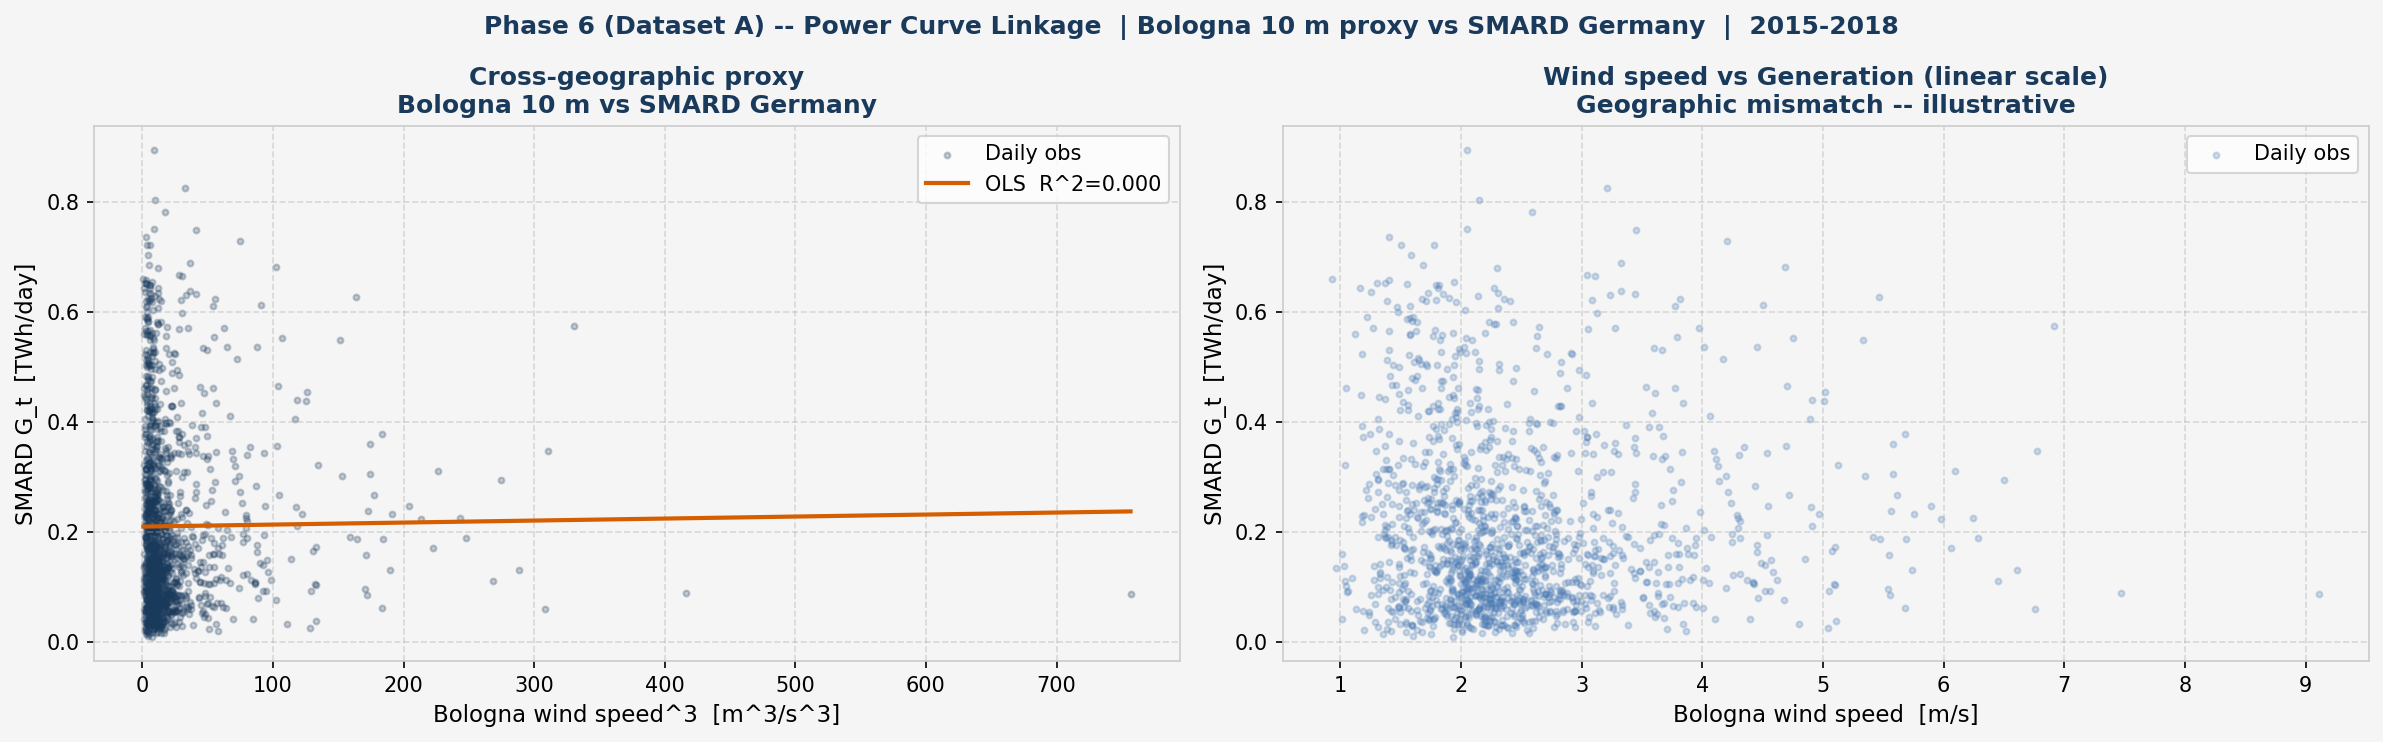
\includegraphics[width=\textwidth]{figures/phase6_A_power_curve.png}
\caption{Dataset A --- Bologna 10~m}
\end{subfigure}
\hfill
\begin{subfigure}{0.40\textwidth}
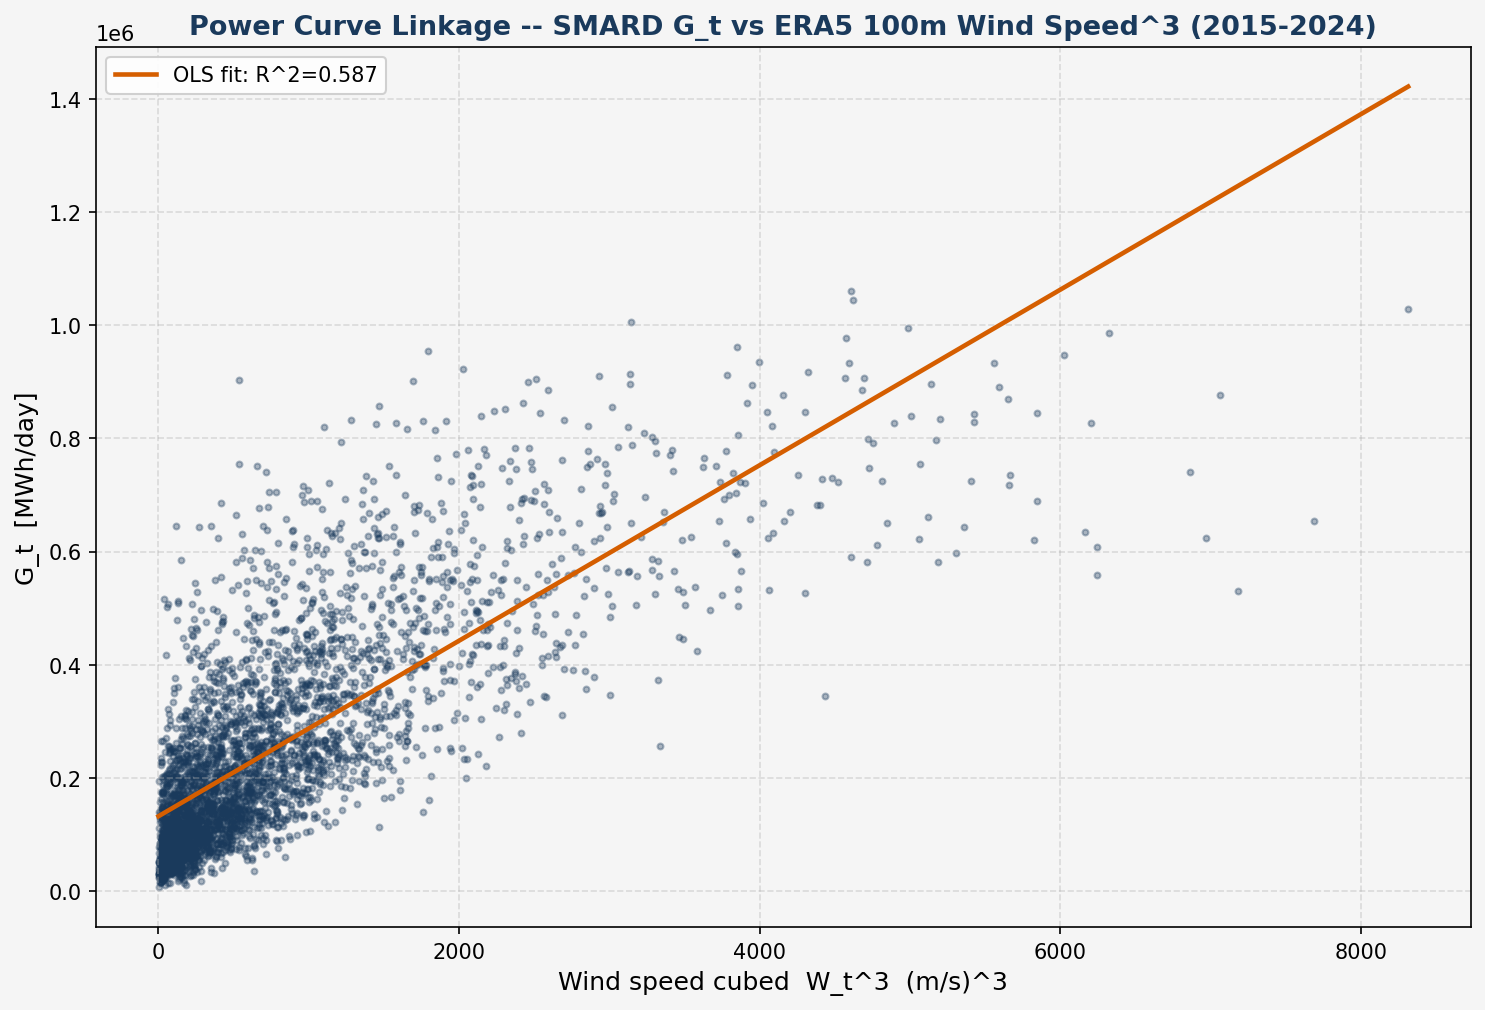
\includegraphics[width=\textwidth]{figures/phase6_B_power_curve.png}
\caption{Dataset B --- Nordfriesland 100~m}
\end{subfigure}
\caption{Power-curve linkage between wind speed and SMARD generation. \textbf{(a)} Dataset~A, two panels: SMARD daily generation in TWh/day against cubed Bologna daily mean wind speed with the fitted ordinary-least-squares line overlaid (left), and the same generation against wind speed on a linear scale (right). The point cloud is structureless in both, consistent with the $R^2 = 0.0001$ of Table~\ref{tab:powercurve}. \textbf{(b)} Dataset~B, a single panel: SMARD daily generation in MWh/day against cubed Nordfriesland 100~m wind speed, with the fitted line. The visible upward slope and the tightening of the cloud along it are the $R^2 = 0.587$ of Table~\ref{tab:powercurve}. Note that the two sub-panels use different axis units and different overlap windows and should be read for the shape of the relation rather than compared point by point.}
\label{fig:powercurve}
\end{figure}

\subsection{The Merit-Order Effect}
\label{sec:merit}

The economic case for a wind-linked hedge rests in part on the relationship between generation and price. Because wind enters the supply stack at near-zero marginal cost, high aggregate wind infeed displaces costlier plant and depresses the day-ahead clearing price. The correlation between daily generation and daily price should therefore be negative, and the analysis is identical for both datasets because both use the same market series.

Over the full 2015--2024 sample the Pearson correlation is $\rho(G,P) = -0.162$. Split at the October~2018 bidding-zone change, it is $-0.476$ on the 1{,}365 days before and $-0.275$ on the 2{,}284 days after. Both sub-periods carry the expected sign, so the merit-order finding survives the structural break, which was the robustness question the split was designed to answer.

The pattern nonetheless deserves more than the robustness verdict. The pooled correlation is weaker in magnitude than either of the sub-period correlations, which is not a possibility that a simple stability check anticipates. The mechanism is a pooling effect: mean price rose from \texteuro{}34.60/MWh over 2015--2020 to \texteuro{}126.47/MWh over 2021--2024 (Section~1.4.3), while installed wind capacity grew steadily across the same window. Pooling the two regimes introduces a large between-regime component into the variance of $P$ that is driven by gas markets rather than by German wind, and that component dilutes the within-regime relationship. The merit-order effect is therefore materially stronger than the headline $-0.162$ suggests, and stronger still in the earlier part of the sample.

The two source documents differ in how they read the sub-period gap: the Dataset~A notebook flags the $0.20$ difference as a divergence to be interpreted with care, the Dataset~B notebook attributes it to growing renewables capacity rather than to the price-zone split. Both readings are consistent with the pooling account above, and neither disturbs the sign, which is the only feature the hedging argument requires.

For a producer, the sign of $\rho$ means that revenue, the product of quantity and price, is less volatile than quantity alone: a partial natural hedge. As Section~1.1 sets out, that hedge is both weak, at $|\rho| = 0.16$ over the full sample, and asymmetric, eroding the upside without placing a floor under the downside. It is the residual volumetric exposure, not the price exposure, that the instruments priced in this chapter address.

\begin{figure}[htbp]
\centering
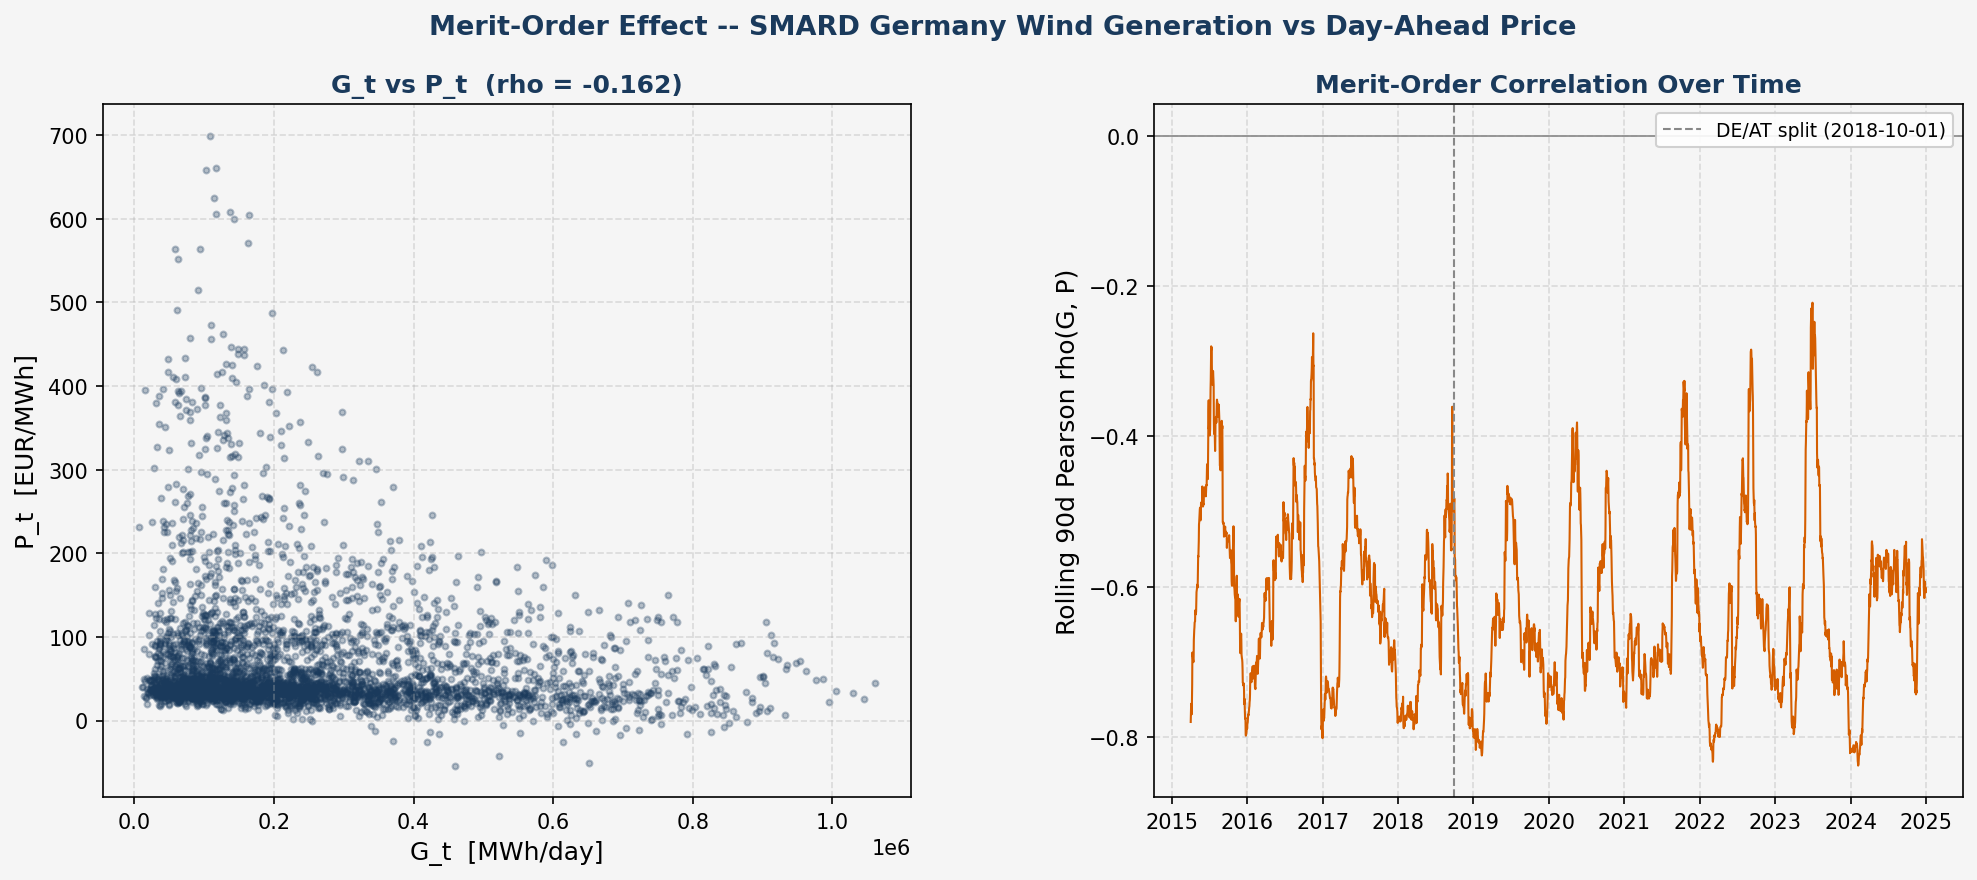
\includegraphics[width=0.9\textwidth]{figures/phase6_B_merit_order.png}
\caption{The merit-order effect. \textbf{Left:} scatter of daily day-ahead price against daily onshore wind generation, 2015--2024, with the full-sample correlation reported in the panel title. \textbf{Right:} the 90-day rolling Pearson correlation between the two series, showing that the relationship is persistently negative but far from constant, and that its magnitude declines over the sample in the way the pooling account of Section~\ref{sec:merit} describes. Both series are market data common to the two datasets, so the figure is shown once.}
\label{fig:merit}
\end{figure}

\subsection{Payoff Simulation}
\label{sec:payoff}

The instrument is evaluated over the ten calendar years of the sample. For each year the annualised realised variance $\mathrm{RV}^{\text{ann}}_y = 252 \times \overline{\mathrm{RV}}_y$ is computed, and the payoff of a unit-notional long position is $\mathrm{RV}^{\text{ann}}_y - K_{\text{var}}$ at each of the candidate strikes. Table~\ref{tab:payoff} reports the annual series.

\begin{table}[htbp]
\centering
\caption{Annual realised variance of SMARD generation log-returns and long variance-swap payoffs at the Track~A strike.}
\label{tab:payoff}
\begin{tabular}{l r r r r}
\toprule
& \multicolumn{2}{c}{\textbf{Dataset A sample}} & \multicolumn{2}{c}{\textbf{Dataset B sample}} \\
\textbf{Year} & \textbf{$\mathrm{RV}^{\text{ann}}$} & \textbf{Payoff} & \textbf{$\mathrm{RV}^{\text{ann}}$} & \textbf{Payoff} \\
\midrule
2015 & $120.83$ & $+6.83$ & $121.62$ & $+8.48$ \\
2016 & $113.23$ & $-0.77$ & $113.23$ & $+0.09$ \\
2017 & $129.17$ & $+15.17$ & $129.17$ & $+16.03$ \\
2018 & $106.16$ & $-7.84$ & $106.16$ & $-6.98$ \\
2019 & $95.49$ & $-18.51$ & $95.49$ & $-17.66$ \\
2020 & $116.74$ & $+2.75$ & $116.74$ & $+3.60$ \\
2021 & $118.97$ & $+4.97$ & $118.97$ & $+5.82$ \\
2022 & $101.80$ & $-12.20$ & $101.80$ & $-11.35$ \\
2023 & $119.71$ & $+5.71$ & $119.71$ & $+6.56$ \\
2024 & $132.00$ & $+18.00$ & $132.00$ & $+18.85$ \\
\midrule
Mean & $115.41$ & $+1.41$ & $115.49$ & $+2.34$ \\
Std.\ deviation & $11.54$ & $11.54$ & $11.59$ & $11.59$ \\
5th percentile & --- & $-15.67$ & --- & $-14.82$ \\
\bottomrule
\end{tabular}
\par\vspace{4pt}
\begin{minipage}{0.92\textwidth}
\footnotesize Payoff is $\mathrm{RV}^{\text{ann}}_y - K_{\text{var}}^A$ for a long unit-notional position; a producer takes the opposite side. Only the 2015 row differs between the two columns, for the alignment reason given in Section~\ref{sec:market-data}. Both Phase~6 source documents tabulate a different set of annual realised variances (Dataset~A: 92.55, 128.41, 120.49, 102.44 for 2015--2018 only; Dataset~B: 95.2 through 106.1 for 2015--2024); neither set appears in either executed notebook, and the values above are the computed ones.
\end{minipage}
\end{table}

Three readings follow. Annual realised variance ranges from $95.5$ in 2019 to $132.0$ in 2024, the highest year exceeding the lowest by 38\% about a mean near $115$, so the quantity being swapped is genuinely variable year to year rather than close to deterministic. The mean payoff at the Track~A strike is small and positive, $+1.41$ and $+2.34$ on the two samples, confirming that a strike set at the full-sample rolling mean was close to fair over the decade; the small positive bias reflects that the rolling estimator lags a mildly upward-trending series. And the fifth-percentile payoff of roughly $-15$ units, against a mean annual level of $115$, quantifies the long party's worst year in the sample at about 13\% of the strike.

The Track~B payoff columns computed in the notebooks, constant at approximately $+115.3$ in every year of both datasets, should not be read as an economic result and are not tabulated here. They are the mechanical consequence of differencing an annualised realised variance of order $115$ against a model strike of order $0.1$: the payoff is simply the realised variance itself, and its apparent risklessness is the units gap of Section~\ref{sec:reconciliation}, not an arbitrage. Once Track~B is reconciled into Track~A units, its Dataset~B value of $328.8$ sits above every annual realisation in Table~\ref{tab:payoff} rather than below all of them, and a producer selling at that strike would have been paid every year of the decade, which is the opposite conclusion and equally a consequence of the model's variance overstatement discussed in Section~\ref{sec:reconciliation}.

\begin{figure}[htbp]
\centering
\begin{subfigure}{0.48\textwidth}
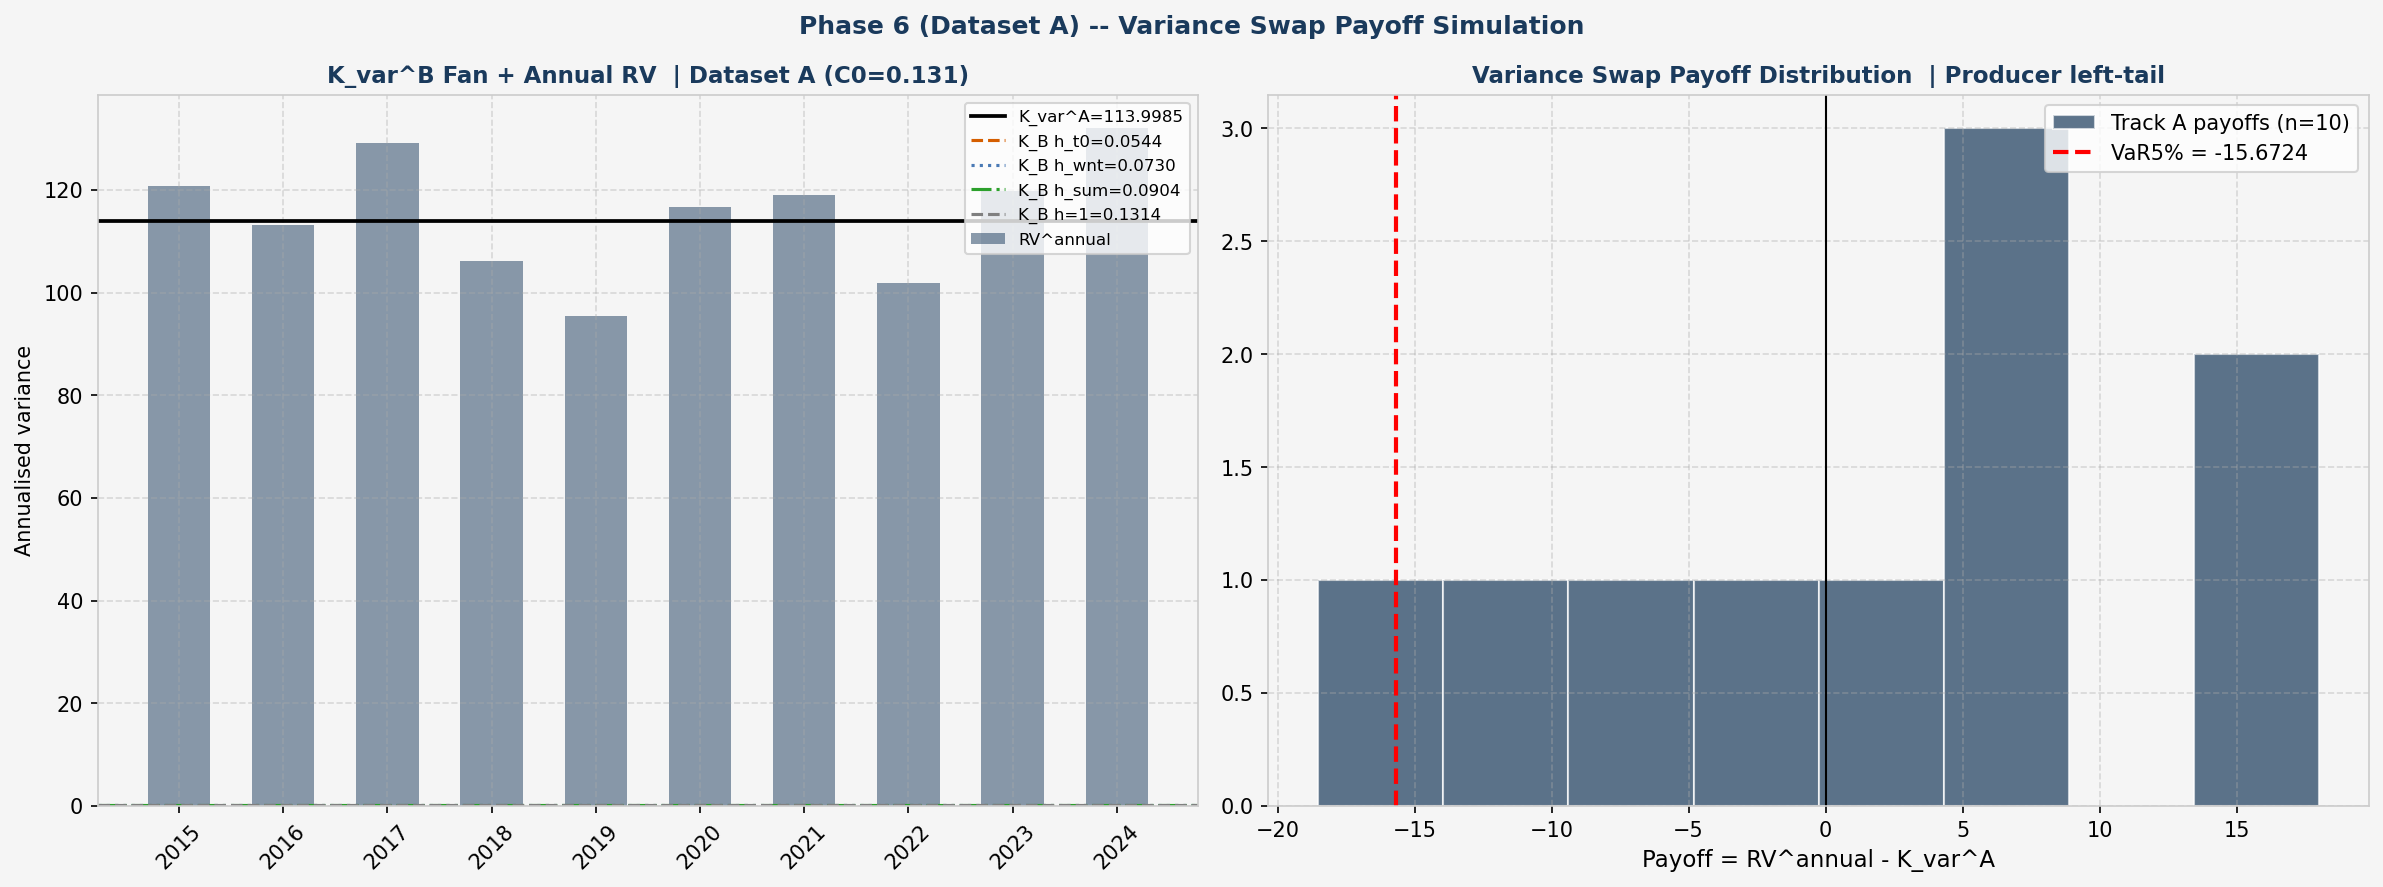
\includegraphics[width=\textwidth]{figures/phase6_A_payoff_fan.png}
\caption{Dataset A}
\end{subfigure}
\hfill
\begin{subfigure}{0.48\textwidth}
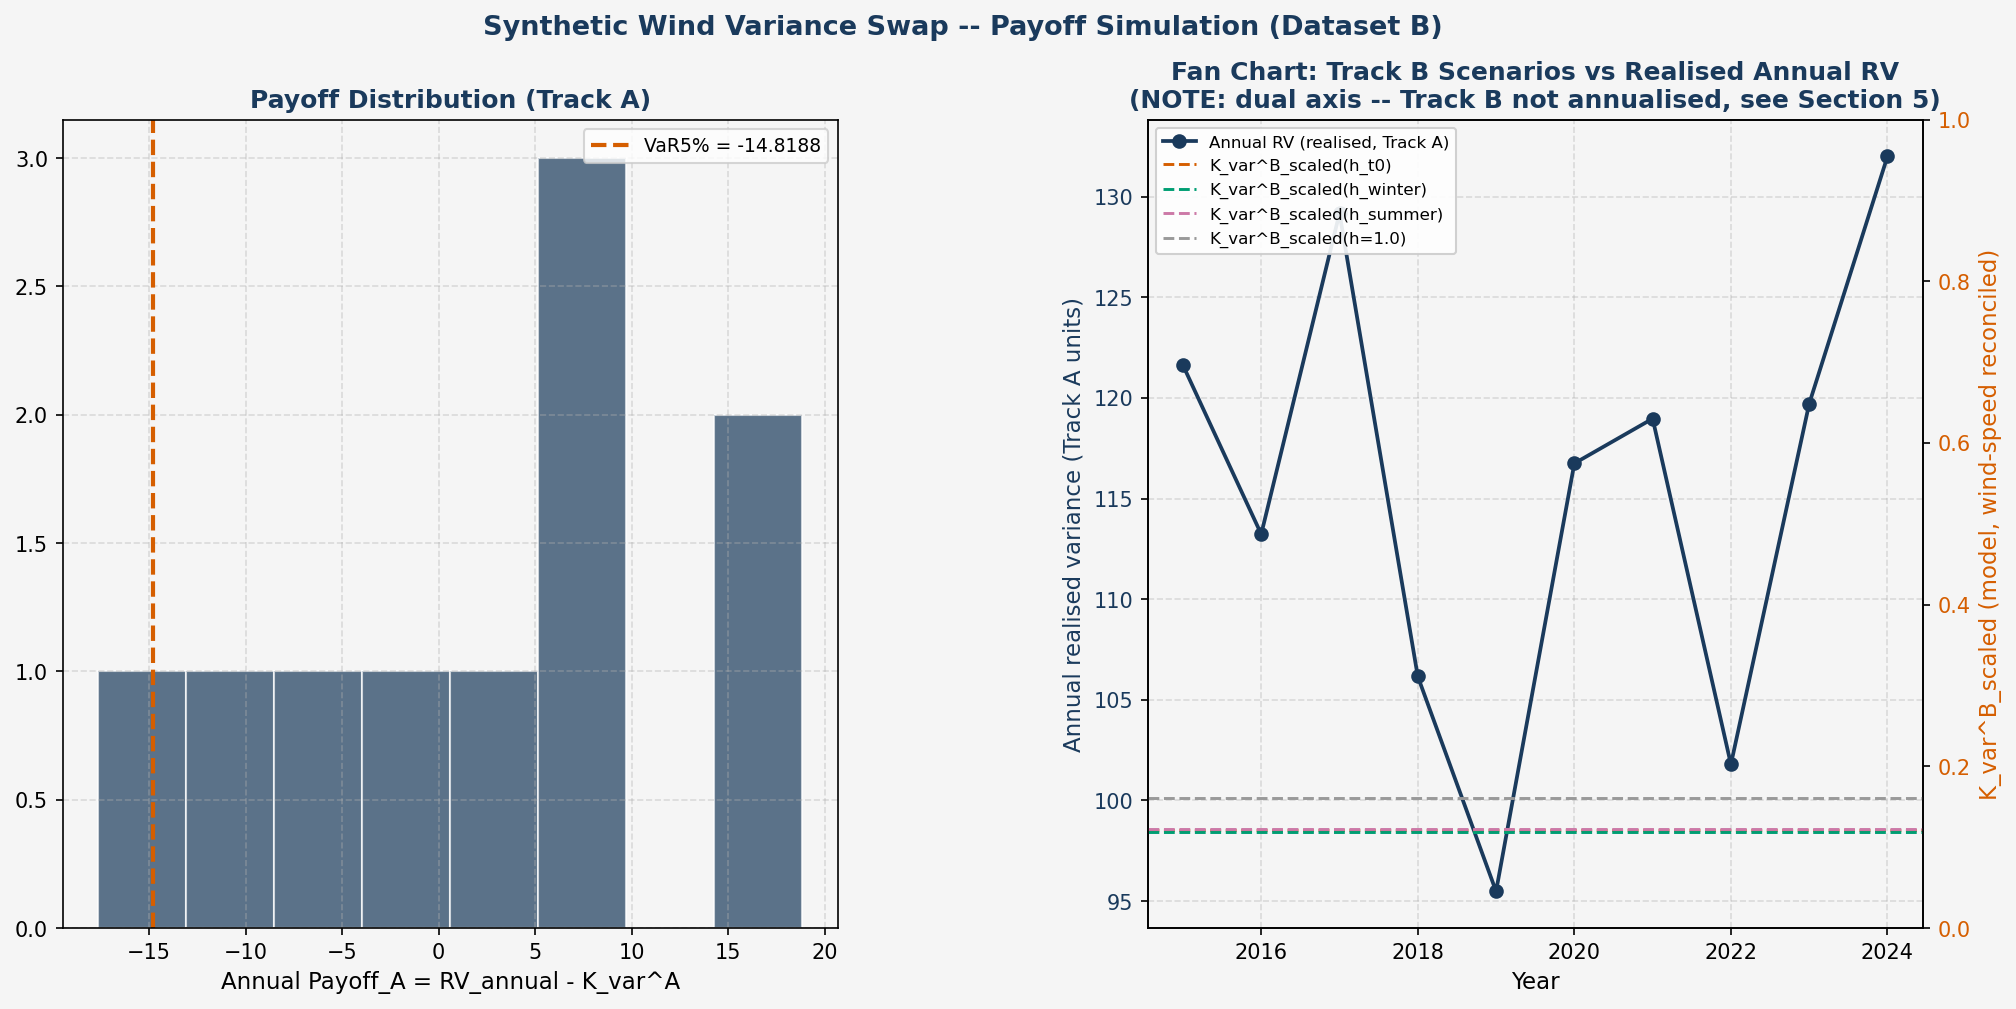
\includegraphics[width=\textwidth]{figures/phase6_B_payoff_fan.png}
\caption{Dataset B}
\end{subfigure}
\caption{Variance-swap payoff simulation, both datasets. \textbf{(a)} Dataset~A, two panels: annual realised variance as bars against the Track~A strike and the four Track~B scenario strikes as horizontal lines (left), and the histogram of the ten annual Track~A payoffs with the fifth percentile marked (right). Because the Track~B lines lie near zero on the annualised axis, they are visually indistinguishable from the horizontal axis, which is the units gap of Section~\ref{sec:reconciliation} rendered graphically. \textbf{(b)} Dataset~B, two panels: the histogram of annual Track~A payoffs with its fifth percentile (left), and a dual-axis fan chart plotting annual realised variance on the left axis against the four unit-reconciled Track~B scenario strikes on the right axis (right). The dual axis is necessary for exactly the reason the Dataset~A panel does not need one, and the panel title in the source figure records the caveat.}
\label{fig:payoff}
\end{figure}

\section{Cross-Dataset Forecast Validation}
\label{sec:validation}

\subsection{The Diebold--Mariano Test and Its Conventions}
\label{sec:dm}

The five specifications developed across Chapters~2 and~3 are compared on one-step-ahead forecasts of the standardised series $\widetilde W(t)$ against a persistence benchmark $\hat{\widetilde W}(t) = \widetilde W(t-1)$, using the test of \citet{DieboldMariano1995} with the small-sample correction of \citet{HarveyEtAl1997}. The loss differential is
\begin{equation}
d_t = e^2_{\text{persistence}}(t) - e^2_{\text{model}}(t),
\end{equation}
so that a model outperforming the benchmark produces a \emph{positive} statistic. This is the reverse of the ordering used in Section~2.2.4, where the model's squared error is differenced first; the two are the same test reaching the same conclusion, and the sign convention is recorded here because the numerical values of the statistic differ in sign between the two chapters. The test statistic is $\bar d / \widehat{\mathrm{se}}(\bar d)$ multiplied by the Harvey--Leybourne--Newbold factor, which at a one-step forecast horizon reduces to $\sqrt{(n-1)/n}$, and referred to a $t$ distribution with $n-1$ degrees of freedom. At the sample sizes involved the correction changes the statistic by about $0.03\%$ and is immaterial to any conclusion; it is applied for correctness rather than for effect.

Two further conventions should be stated. First, the evaluation is conducted on the full standardised sample using the frozen Phase~2 residuals, not on a held-out partition, which is why the root mean squared errors below differ from those of Table~2.6. Second, the AR(4)+GARCH, CAR(4)+Gaussian and CAR(4)+NIG specifications enter the test with error series set identically equal to the AR(4) errors. This is not a coding shortcut but the implementation of the argument made in Section~2.2.4: the GARCH layer models the conditional variance of the residuals, the CAR(4) embedding is an exact continuous-time representation of the same mean dynamics, and a symmetric NIG innovation has the same conditional mean as a Gaussian one, so none of the three alters the one-step point forecast. The consequence is that their RMSE, DM statistic and $p$-value are identical to AR(4)'s by construction rather than by empirical coincidence, and no inference about their relative merit can be drawn from this table.

\subsection{Results}
\label{sec:dm-results}

\begin{table}[htbp]
\centering
\caption{Diebold--Mariano tests against the persistence benchmark, one-step-ahead forecasts of $\widetilde W(t)$, full sample.}
\label{tab:dm}
\begin{tabular}{l r r r r}
\toprule
& \multicolumn{2}{c}{\textbf{Dataset A}} & \multicolumn{2}{c}{\textbf{Dataset B}} \\
\textbf{Model} & \textbf{RMSE} & \textbf{DM stat} & \textbf{RMSE} & \textbf{DM stat} \\
\midrule
Persistence (benchmark) & $0.8868$ & --- & $1.0046$ & --- \\
AR(4) & $0.7802$ & $8.265$ & $0.8681$ & $16.758$ \\
AR(4)+GARCH & $0.7802$ & $8.265$ & $0.8681$ & $16.758$ \\
CAR(4)+Gaussian & $0.7802$ & $8.265$ & $0.8681$ & $16.758$ \\
CAR(4)+NIG & $0.7802$ & $8.265$ & $0.8681$ & $16.758$ \\
\midrule
Improvement over persistence & \multicolumn{2}{c}{$12.0\%$} & \multicolumn{2}{c}{$13.6\%$} \\
$p$-value & \multicolumn{2}{c}{$4.4\times10^{-16}$} & \multicolumn{2}{c}{$<10^{-16}$} \\
\bottomrule
\end{tabular}
\par\vspace{4pt}
\begin{minipage}{0.92\textwidth}
\footnotesize The three specifications below AR(4) share its error series by construction (Section~\ref{sec:dm}); their identical entries record that fact and are not independent evidence.
\end{minipage}
\end{table}

Table~\ref{tab:dm} reports the outcome. Every fitted specification rejects equality of predictive accuracy with persistence at any conventional level, with relative improvements of 12.0\% for Dataset~A and 13.6\% for Dataset~B. The result is therefore a binary split rather than a graded hierarchy, exactly as anticipated in Section~1.5: the models beat the naive benchmark decisively and are observationally equivalent to one another at a one-day horizon by construction.

The two datasets' absolute figures differ, and both differences are accounted for. The root mean squared errors here (Dataset~A: $0.7802$ and $0.8868$) exceed those of Table~2.6 (Dataset~A: $0.6017$ and $0.6856$) because the present evaluation uses the full sample rather than the held-out partition. For Dataset~B the two evaluations nearly coincide ($0.8681$ against $0.8580$, and $1.0046$ against $0.9955$, both within 1\%), while for Dataset~A they differ by 23\%. That asymmetry is itself informative and is consistent with the conditional-variance profiles of Section~2.3.1: Dataset~A's held-out window sits at the end of a sample where $h(t_0) = 0.4137$ against an unconditional level of $0.608$, and $\sqrt{0.4137/0.608} = 0.825$ is close to the observed ratio of $0.773$, whereas Dataset~B's $h(t_0) = 0.7511$ sits at its unconditional $0.7522$ and predicts a ratio of essentially one against the observed $0.991$. The held-out partition was, for Dataset~A alone, an unusually calm period.

The Diebold--Mariano statistics stand at $8.265$ and $16.758$, a ratio of $2.03$. A DM statistic scales with the square root of the evaluation sample, and $\sqrt{3652/1461} = 1.58$ accounts for most of it; the residual factor of $1.28$ is consistent with Dataset~B's larger relative accuracy gain and lower loss-differential dispersion. The Dataset~B phase document reads the full $2.03$ as evidence that ``the improvement in AR(4) is also genuinely larger,'' which is directionally right but overstates the residual once the sample-size effect is removed. Section~2.2.4 performs the equivalent decomposition for the held-out statistics and reaches the same conclusion by the same route.

\begin{figure}[htbp]
\centering
\begin{subfigure}{0.48\textwidth}
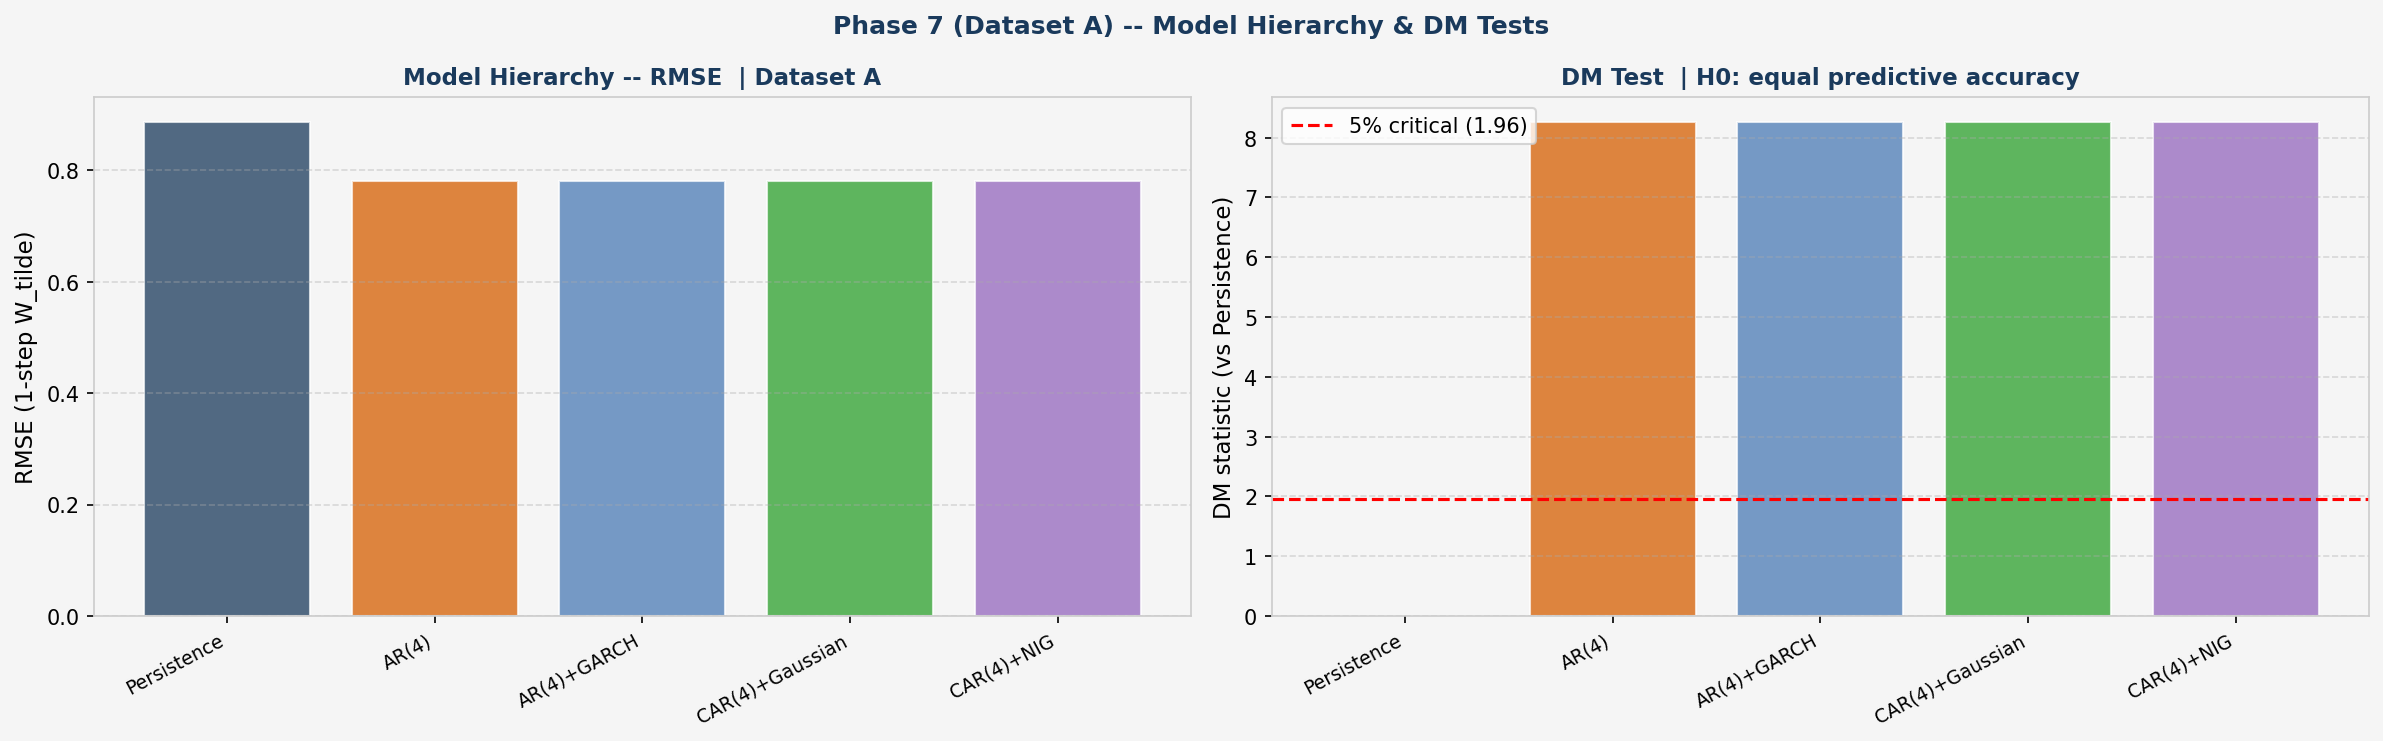
\includegraphics[width=\textwidth]{figures/phase7_A_dm_tests.png}
\caption{Dataset A}
\end{subfigure}
\hfill
\begin{subfigure}{0.48\textwidth}
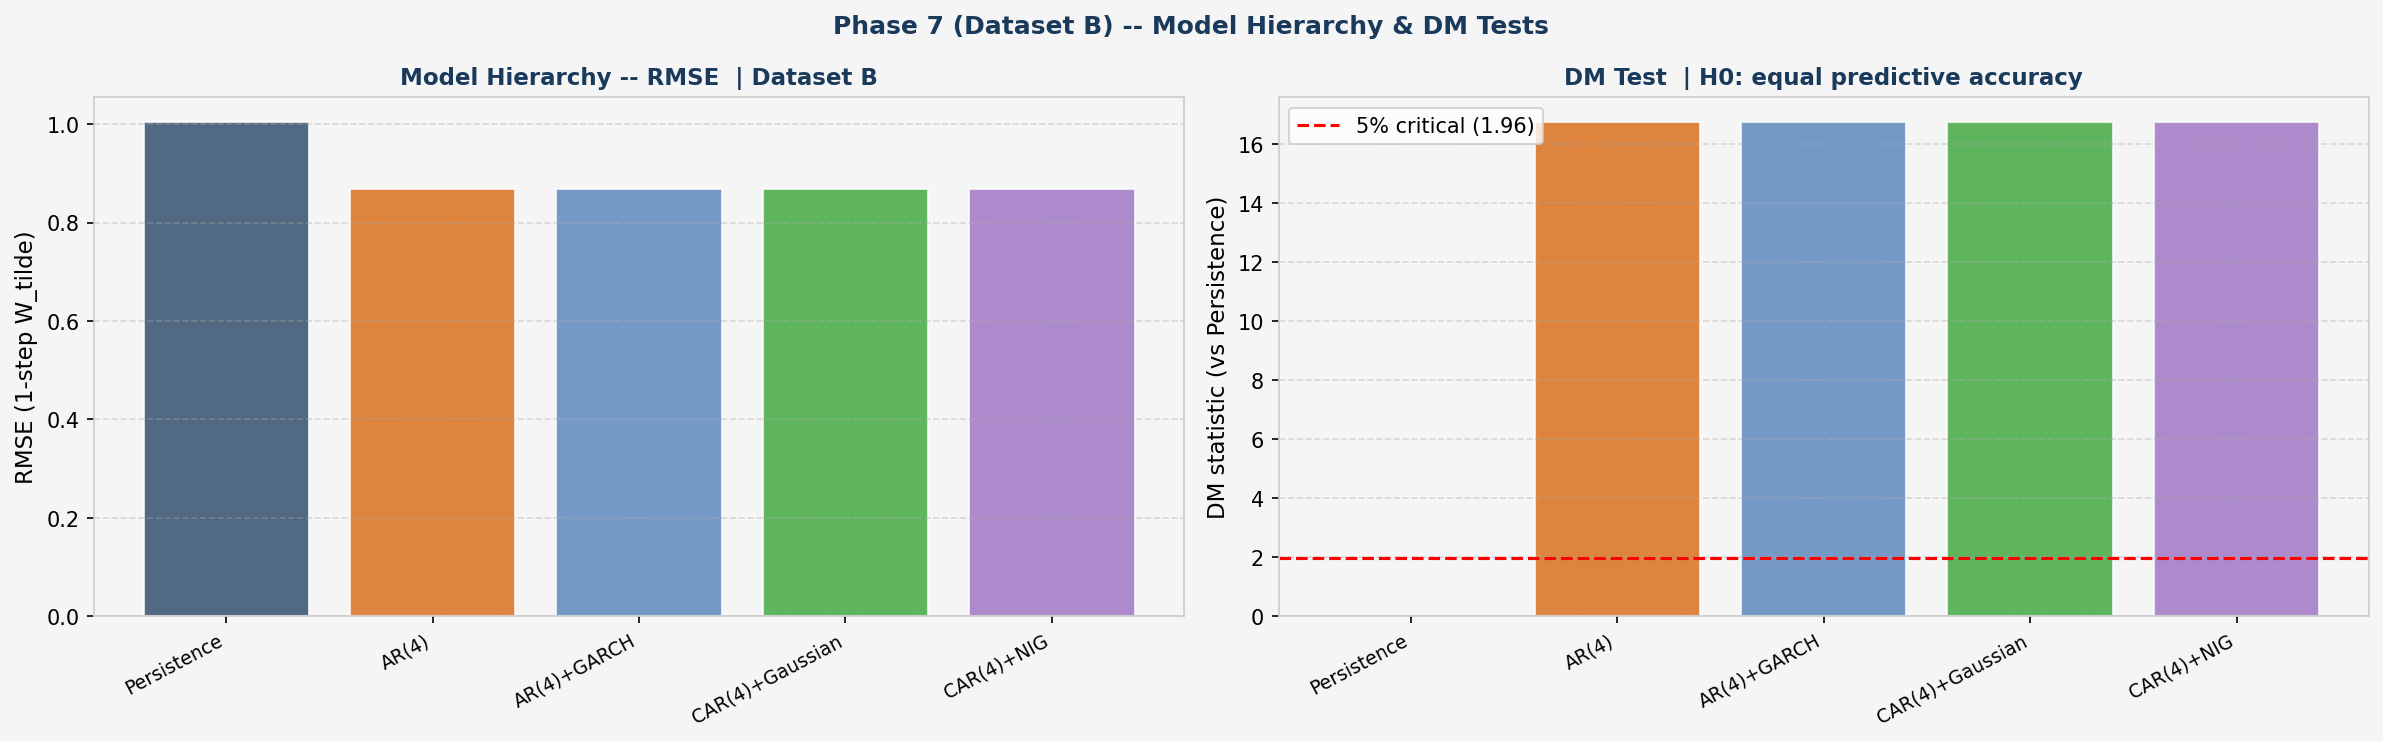
\includegraphics[width=\textwidth]{figures/phase7_B_dm_tests.png}
\caption{Dataset B}
\end{subfigure}
\caption{Model hierarchy and Diebold--Mariano tests, both datasets. Each panel has two plots. \textbf{Left:} one-step-ahead root mean squared error on $\widetilde W(t)$ as a bar per model, with the persistence benchmark distinguished; the four fitted bars are of equal height for the construction reason given in Section~\ref{sec:dm}. \textbf{Right:} the corresponding Diebold--Mariano statistics as bars, with the two-sided 5\% critical value of $1.96$ marked as a horizontal reference line, against which every fitted model stands several times higher.}
\label{fig:dm}
\end{figure}

\subsection{GARCH Volatility Diagnostics}
\label{sec:garch-diag}

The adequacy of the \citet{Bollerslev1986} GARCH(1,1) layer is re-examined on the standardised residuals $z(t) = \hat\varepsilon(t)/\sqrt{h(t)}$, using Ljung--Box tests on $z(t)$ and $z(t)^2$ at lags 5, 10 and 20 and the Engle \citeyearpar{Engle1982} Lagrange-multiplier test at lag 5. Table~\ref{tab:garch-diag} reports the results.

\begin{table}[htbp]
\centering
\caption{GARCH(1,1) standardised-residual diagnostics, $p$-values, both datasets.}
\label{tab:garch-diag}
\begin{tabular}{l r r}
\toprule
\textbf{Test} & \textbf{Dataset A} & \textbf{Dataset B} \\
\midrule
Ljung--Box $z(t)$, lag 5 & $0.9307$ & $0.9820$ \\
Ljung--Box $z(t)$, lag 10 & $0.9896$ & $0.5305$ \\
Ljung--Box $z(t)$, lag 20 & $0.7762$ & $0.5112$ \\
\midrule
Ljung--Box $z(t)^2$, lag 5 & $0.8196$ & $\mathbf{0.0167}$ \\
Ljung--Box $z(t)^2$, lag 10 & $0.9790$ & $0.0810$ \\
Ljung--Box $z(t)^2$, lag 20 & $0.9886$ & $0.2863$ \\
\midrule
ARCH-LM, lag 5 & $0.8212$ & $\mathbf{0.0185}$ \\
\bottomrule
\end{tabular}
\par\vspace{4pt}
\begin{minipage}{0.92\textwidth}
\footnotesize Bold entries reject at 5\%. These figures reproduce the lag-20 and ARCH-LM values reported in Table~2.9 to within rounding, the Dataset~B ARCH-LM statistic exactly.
\end{minipage}
\end{table}

For Dataset~A the verdict is unambiguous: every test passes comfortably, with no $p$-value below $0.77$, and GARCH(1,1) has removed both the serial correlation and the conditional heteroskedasticity present in the AR(4) residuals. For Dataset~B the picture is more qualified. The level tests pass at every lag, but the squared-residual test rejects at lag 5 ($p = 0.0167$), is marginal at lag 10 ($p = 0.0810$), and passes at lag 20 ($p = 0.2863$), while the ARCH-LM test rejects at 5\% ($p = 0.0185$). Some short-lag volatility structure therefore survives the GARCH filter in the reference dataset.

This finding is not new to the present chapter: Section~2.3.3 identified the same ARCH-LM rejection and noted that the Phase~7 recomputation returns the identical statistic. It is restated here for two reasons. The first is that both Phase~7 source documents record the Dataset~B residuals as passing all diagnostics with $p > 0.05$, a characterisation their own executed output contradicts at two of the seven tests reported above. The second is that the rejection is at short lags only, which points to a specific and remediable limitation rather than to a failure of the specification: a GARCH(1,1) has a single decay rate and cannot simultaneously match a fast component operating over a few days and the slow, roughly 38-day component that dominates Dataset~B's persistence (Section~2.3.1). A two-component or GARCH(2,1) specification would be the natural response. That extension is not pursued here, because the pricing formula of Section~\ref{sec:trackb} uses only $h(t_0)$ and the unconditional level, neither of which is materially altered by short-lag misfit, but the diagnostic should be reported as it stands rather than as it was described.

\begin{figure}[htbp]
\centering
\begin{subfigure}{0.48\textwidth}
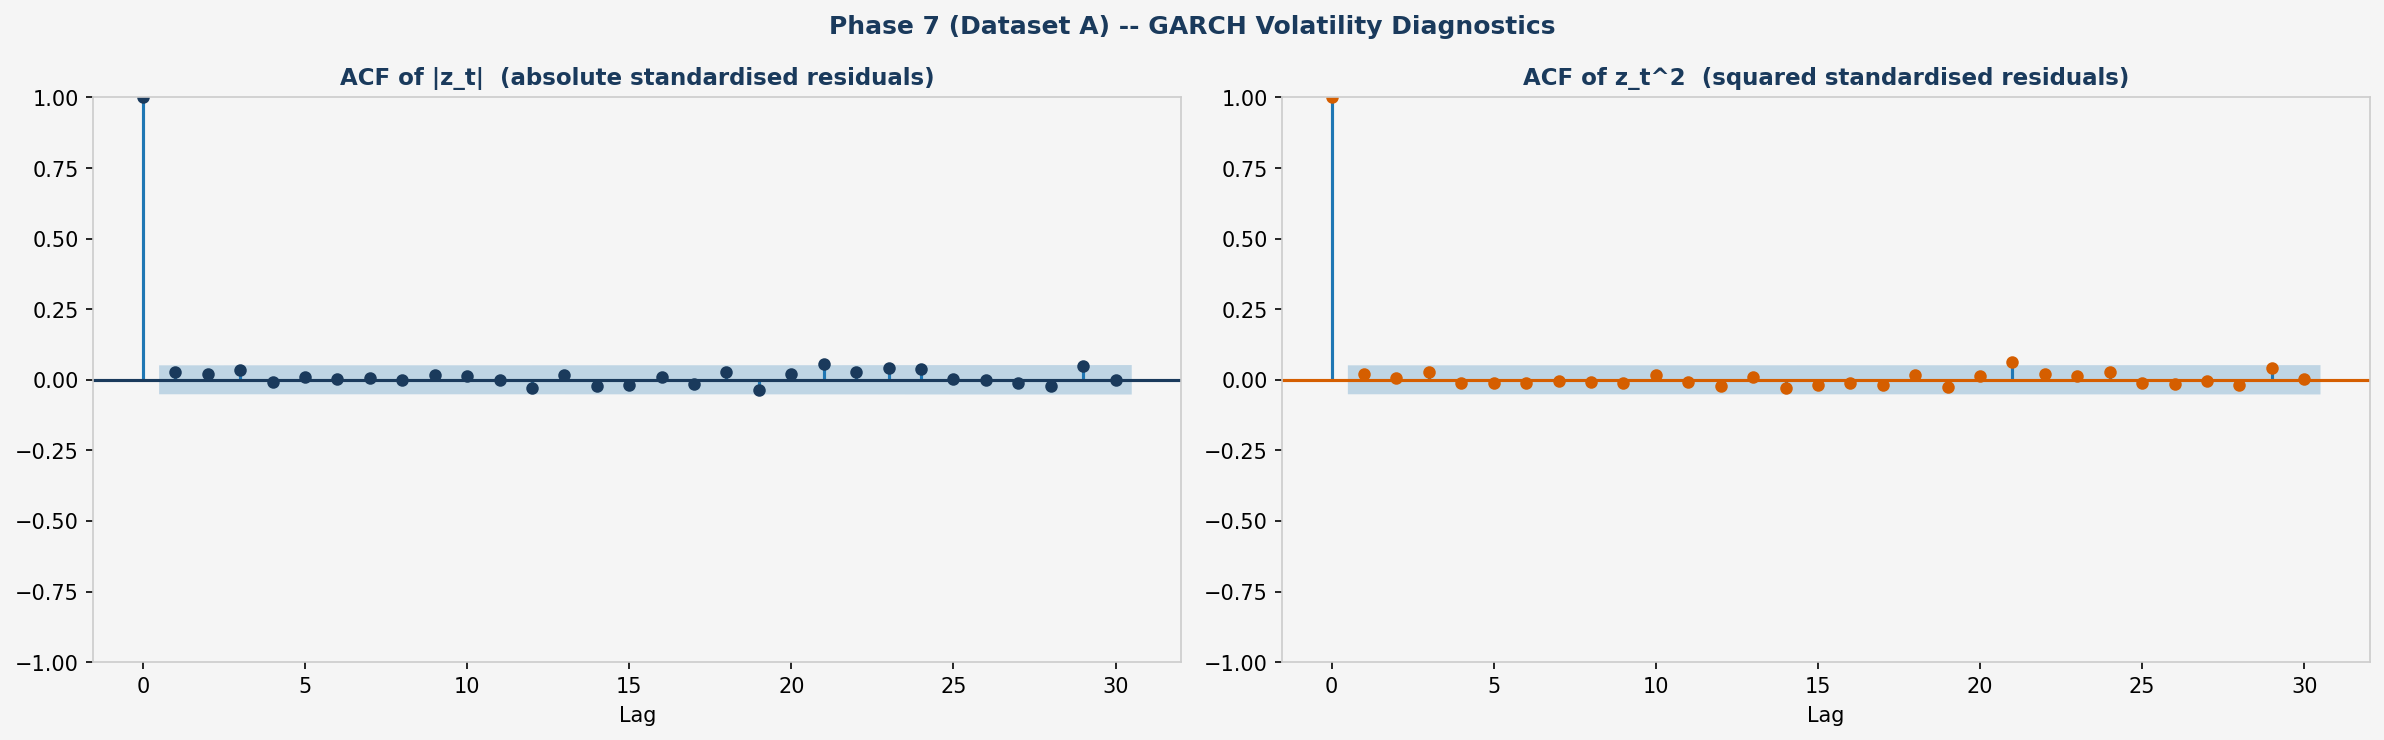
\includegraphics[width=\textwidth]{figures/phase7_A_garch_diagnostics.png}
\caption{Dataset A}
\end{subfigure}
\hfill
\begin{subfigure}{0.48\textwidth}
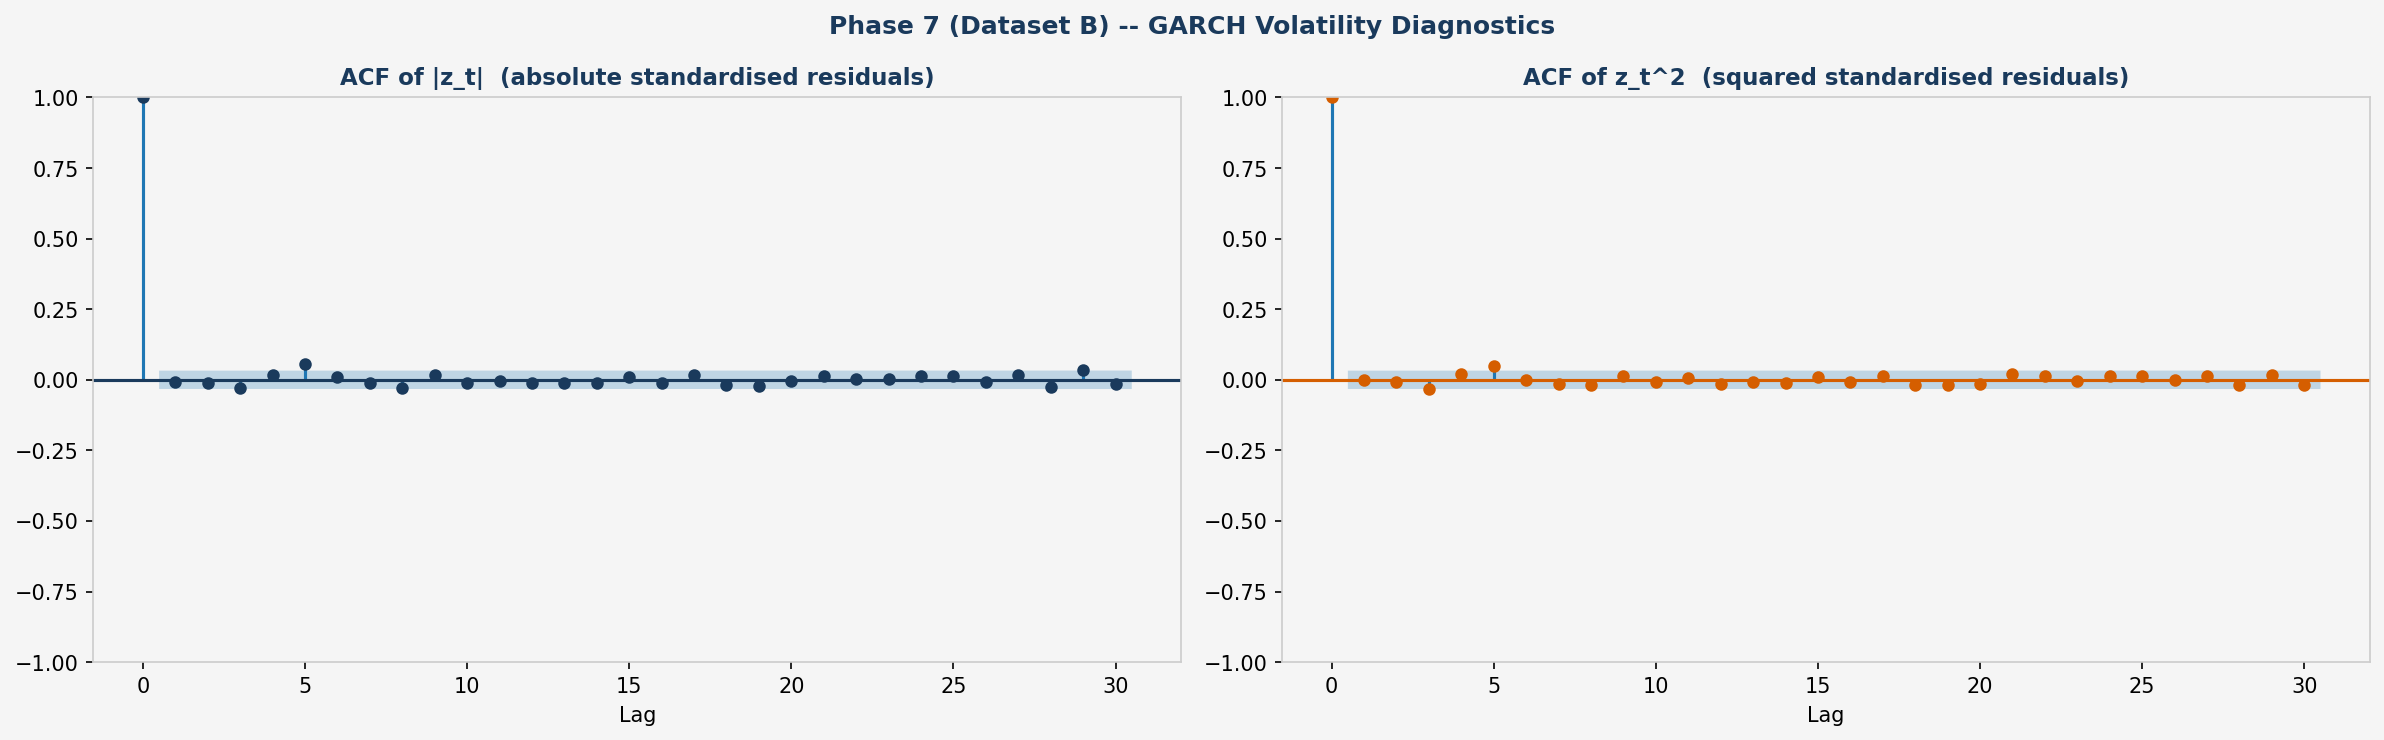
\includegraphics[width=\textwidth]{figures/phase7_B_garch_diagnostics.png}
\caption{Dataset B}
\end{subfigure}
\caption{GARCH standardised-residual autocorrelation diagnostics, both datasets. Each panel has two plots: the sample autocorrelation function of $|z(t)|$ (left) and of $z(t)^2$ (right), the two standard graphical checks for residual volatility clustering. Bars falling inside the confidence band indicate that the corresponding lag carries no remaining structure. Dataset~B's short-lag bars in the right-hand plot are the graphical counterpart of the lag-5 rejections in Table~\ref{tab:garch-diag}.}
\label{fig:garch-diag}
\end{figure}

\subsection{Forecast-Error Distribution}
\label{sec:forecast-dist}

The one-day-ahead forecast errors of each specification are tested for normality by the Jarque--Bera statistic. Table~\ref{tab:jb} reports the outcome.

\begin{table}[htbp]
\centering
\caption{Jarque--Bera tests on one-day-ahead forecast errors.}
\label{tab:jb}
\begin{tabular}{l r r r r}
\toprule
& \multicolumn{2}{c}{\textbf{Dataset A}} & \multicolumn{2}{c}{\textbf{Dataset B}} \\
\textbf{Model} & \textbf{JB} & \textbf{$p$} & \textbf{JB} & \textbf{$p$} \\
\midrule
Persistence & $59.96$ & $<0.001$ & $0.756$ & $0.685$ \\
AR(4) & $108.87$ & $<0.001$ & $17.05$ & $<0.001$ \\
CAR(4)+Gaussian & $108.87$ & $<0.001$ & $17.05$ & $<0.001$ \\
CAR(4)+NIG & $108.87$ & $<0.001$ & $17.05$ & $<0.001$ \\
\bottomrule
\end{tabular}
\end{table}

The three fitted rows are identical for the construction reason given in Section~\ref{sec:dm}. It is worth noting that they would be identical even if the NIG variant had been implemented as its source document describes, namely by dividing the AR(4) residuals by the scale parameter $\hat\delta = 2.087$ of the Normal-Inverse-Gaussian fit of \citet{BarndorffNielsenShephard2001} reported in Section~2.4.4: the Jarque--Bera statistic depends only on the third and fourth standardised moments and is therefore invariant to any change of location or scale. Dividing a residual series by a constant cannot change its skewness or its kurtosis, and so cannot change its Jarque--Bera $p$-value. The Dataset~A phase document nevertheless reports a Jarque--Bera statistic of $3.7$ with $p = 0.1596$ for the NIG variant and concludes that ``NIG normalisation succeeds''; that figure appears nowhere in the executed output, and the claim is not merely unsupported but not the kind of claim the stated procedure could support.

The substantive content of the table lies in the other two results. Both datasets' fitted residuals reject normality, Dataset~A decisively ($\mathrm{JB} = 108.9$) and Dataset~B more mildly ($\mathrm{JB} = 17.0$), which is the same ordering found for the GARCH standardised residuals in Section~2.4.4: Dataset~A is leptokurtic and driven substantially by the single $5.79\sigma$ event of 28~June~2017, Dataset~B only slightly non-Gaussian. And Dataset~B's persistence errors are, uniquely in the table, indistinguishable from normal ($\mathrm{JB} = 0.756$, $p = 0.685$). The most likely explanation is that a first difference is the sum of two draws of opposite sign from a serially dependent series, and such a sum is closer to Gaussian than either component; the AR(4) innovation, by contrast, isolates the raw shock and preserves whatever non-normality it carries. This is offered as an interpretation of the pattern rather than as a separately tested result.

Two scope notes complete the section. The forecast-error analysis specified for this phase called for residuals at horizons of 1, 7 and 14 days and for quantile--quantile comparison against both the Normal and the NIG distributions. What was implemented is the one-day horizon only, compared against the Normal alone, in both datasets. The multi-horizon and NIG-quantile comparisons are therefore not available, and the question of whether the NIG assumption offers a statistically significant improvement over the Gaussian is not answered by this evidence. The answer it would have given is nevertheless partly foreshadowed by Section~2.4.4, where the NIG fit to Dataset~A's standardised residuals improved the Kolmogorov--Smirnov $p$-value from $0.079$ to $0.120$, a modest gain, while for Dataset~B the fitted tail parameter $\hat\alpha \approx 2{,}650$ left the NIG indistinguishable from the Gaussian. The Gaussian CAR(4) specification is retained as the primary pricing track for both datasets on that basis.

\begin{figure}[htbp]
\centering
\begin{subfigure}{0.48\textwidth}
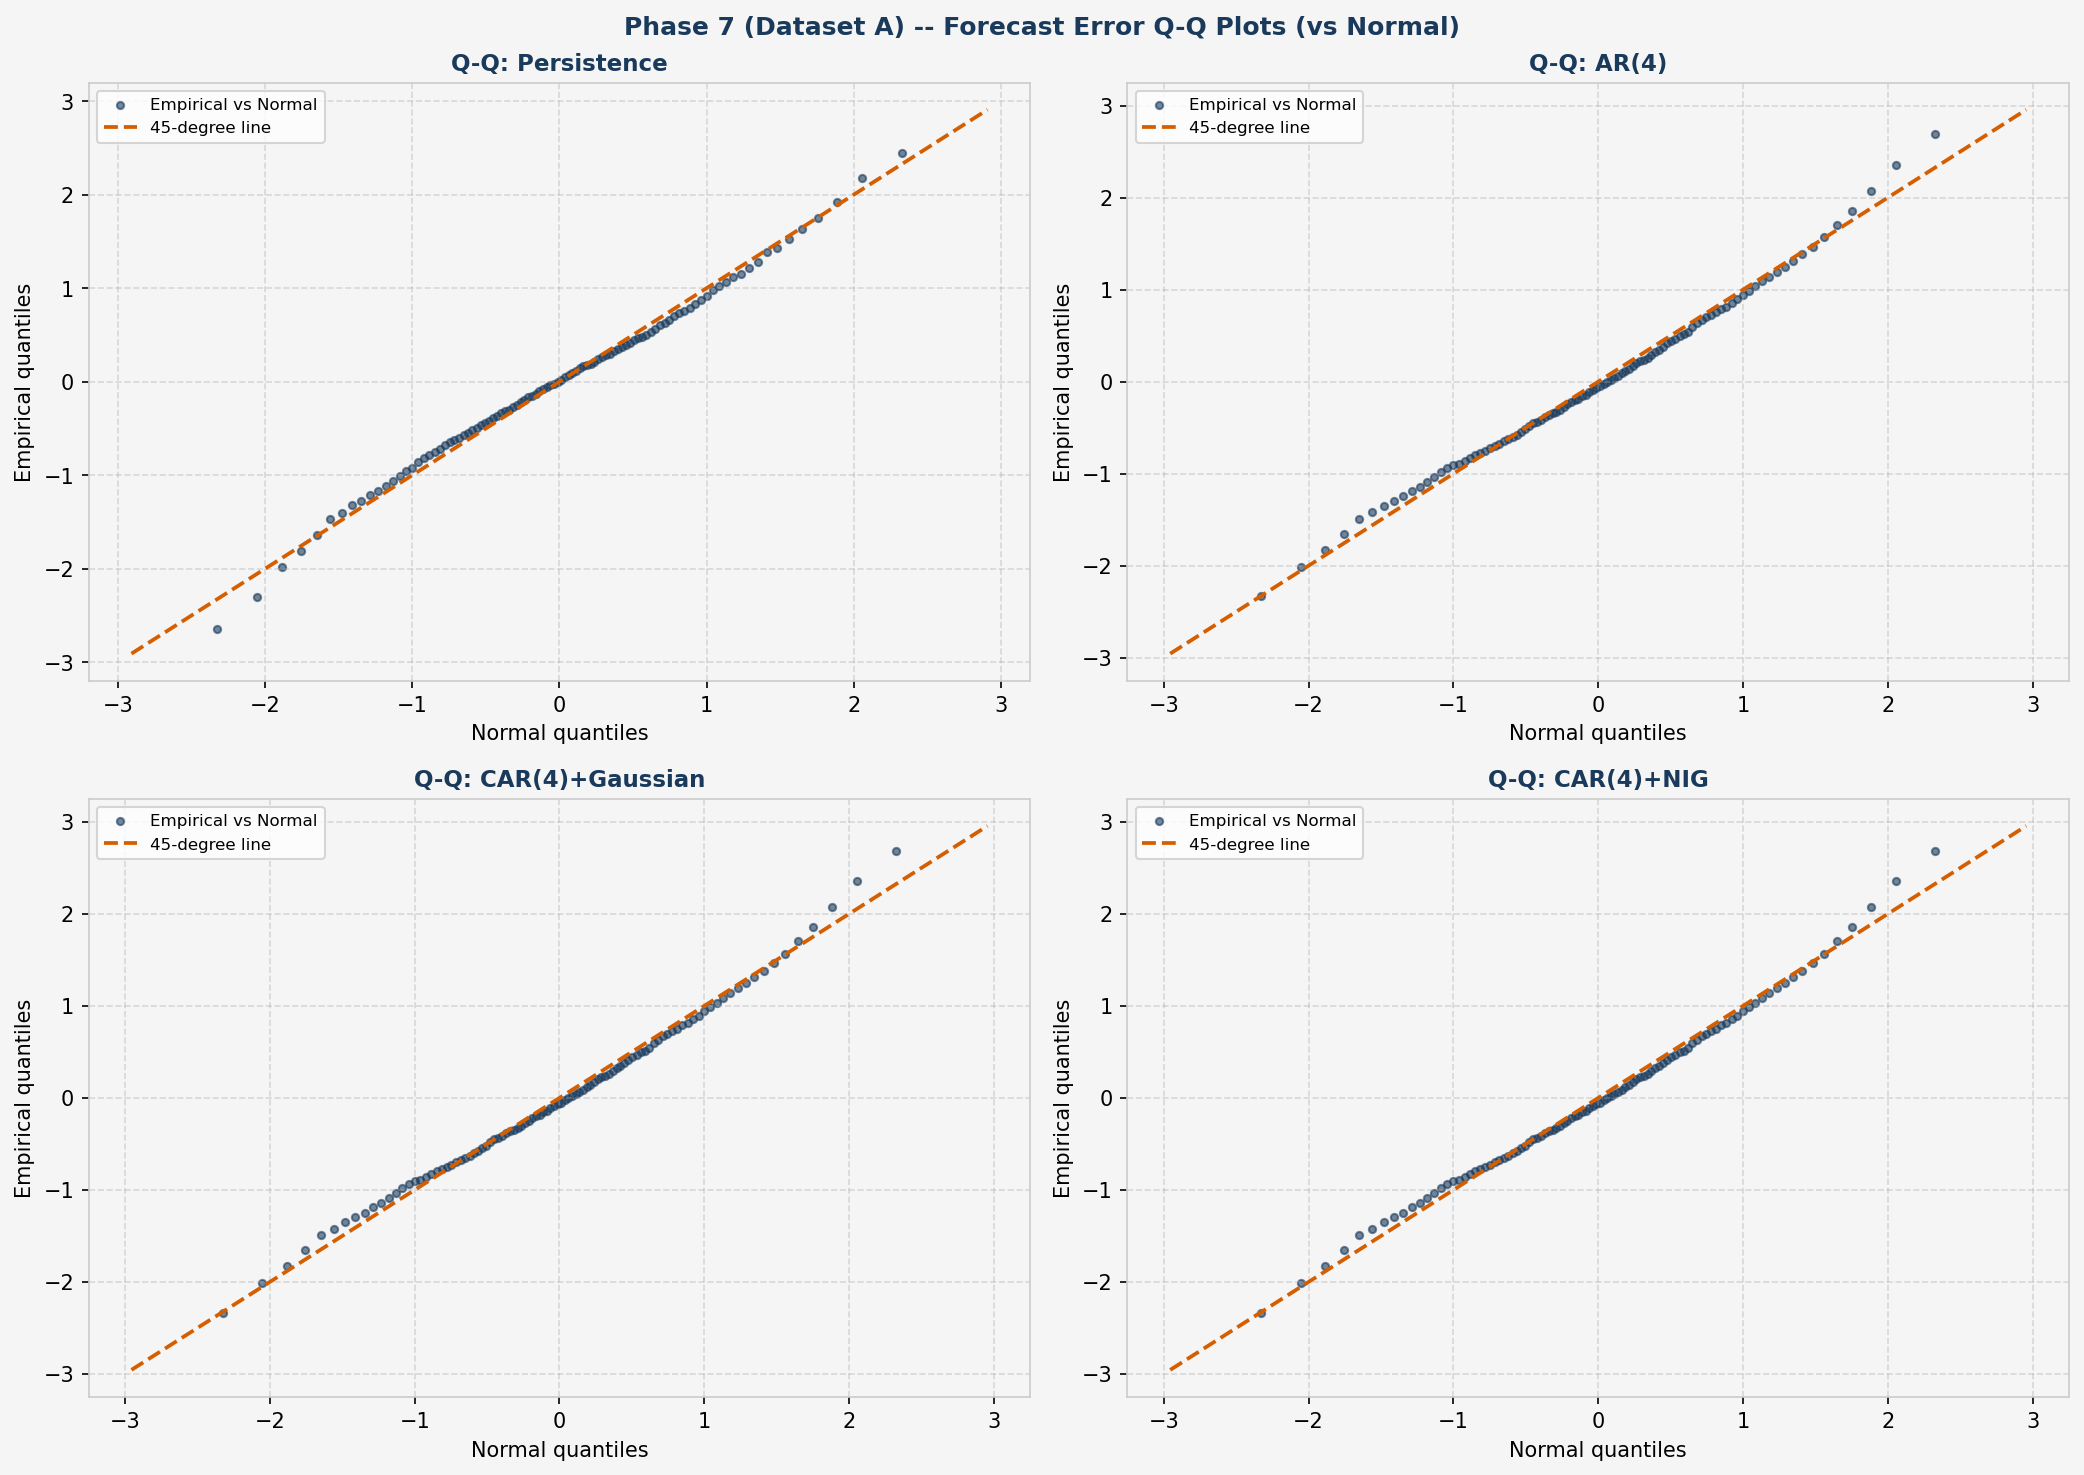
\includegraphics[width=\textwidth]{figures/phase7_A_forecast_dist.png}
\caption{Dataset A}
\end{subfigure}
\hfill
\begin{subfigure}{0.48\textwidth}
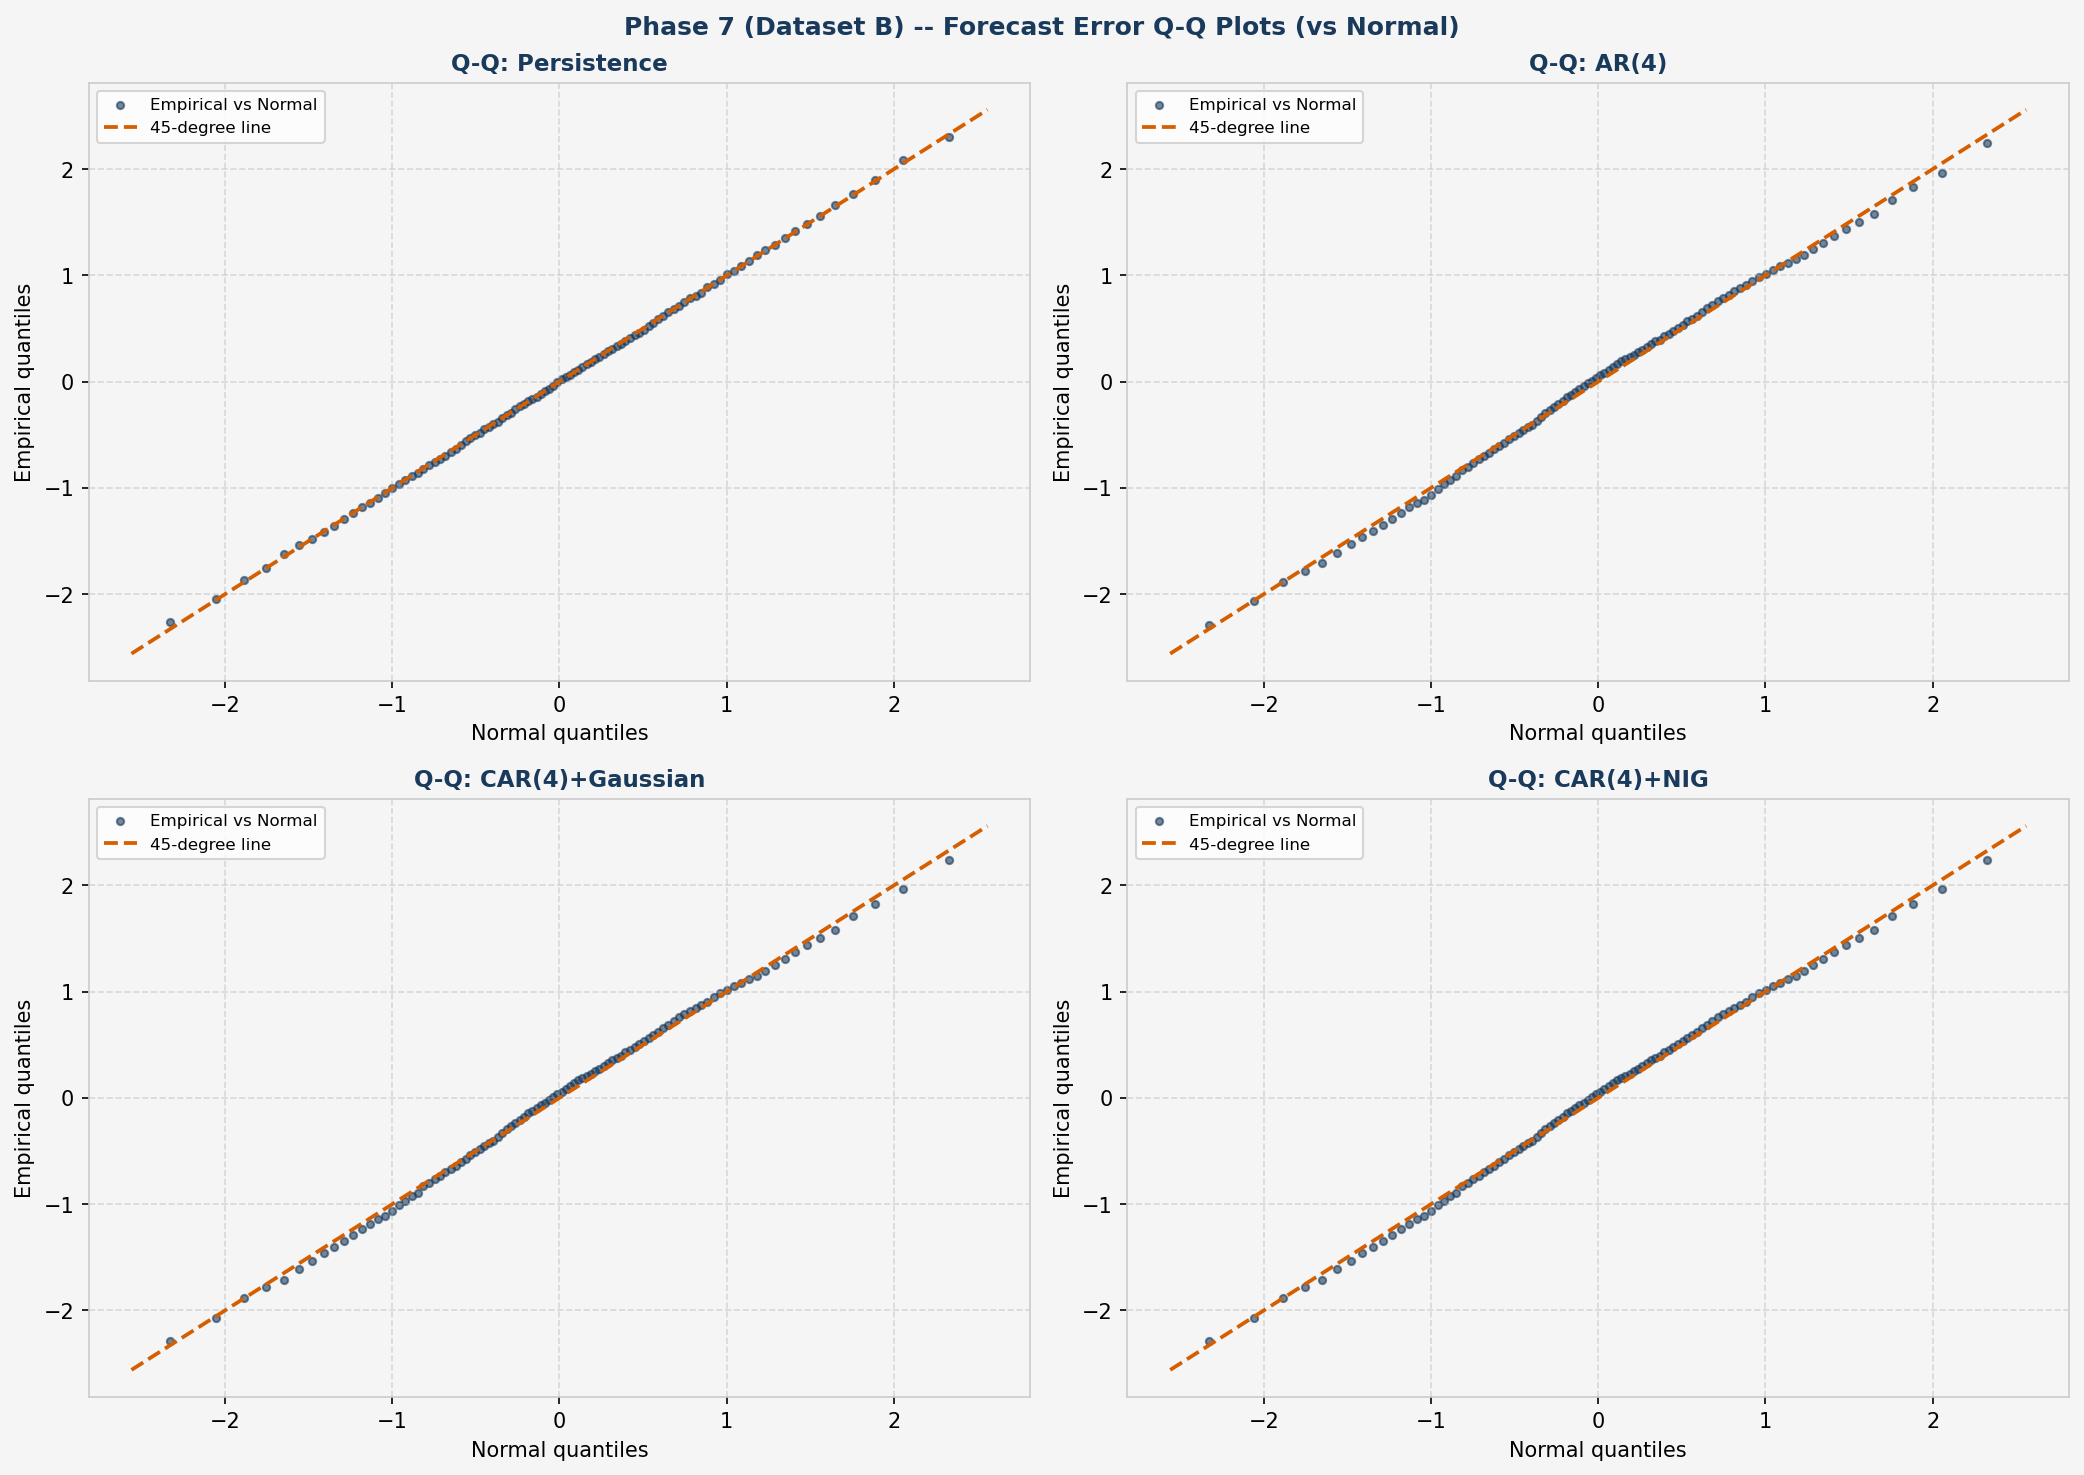
\includegraphics[width=\textwidth]{figures/phase7_B_forecast_dist.png}
\caption{Dataset B}
\end{subfigure}
\caption{Quantile--quantile plots of one-day-ahead forecast errors against the normal distribution, both datasets. Each panel is a $2\times2$ grid, one plot per model in the order persistence, AR(4), CAR(4)+Gaussian, CAR(4)+NIG, with the empirical quantiles of the standardised errors plotted against normal quantiles and the 45-degree line overlaid. Because the errors are standardised before plotting and the three fitted models share one error series, their three plots are identical within each panel; only the persistence plot differs. Departure from the 45-degree line at the extremes is the leptokurtosis quantified in Table~\ref{tab:jb}, pronounced for Dataset~A and slight for Dataset~B.}
\label{fig:forecast-dist}
\end{figure}

\section{Value of Information}
\label{sec:voi}

\subsection{The Height Correction}
\label{sec:height}

The two datasets are measured at different heights, so a comparison of their implied strikes must either adjust for height or acknowledge that it has not. The adjustment used is the power-law profile of \citet{PetersonHennessey1978}, $u(z) \propto z^{\alpha}$ with $\alpha = 1/7$; since variance scales as the square of velocity, the variance correction from 10~m to 100~m is
\begin{equation}
\left(\frac{100}{10}\right)^{2\alpha} = 10^{2/7} = 1.9307.
\label{eq:height}
\end{equation}
As stipulated in Section~1.3.1, this factor is applied in this section and nowhere else in the thesis: Dataset~B is already at hub height and requires no correction, and no other calculation in Chapters~2 or~3 places the two datasets on a common vertical axis. The exponent is empirical rather than physical, varying with surface roughness and atmospheric stability from about $1/10$ over open water to substantially more over rough terrain, and a coastal German site sits near the middle of that range; a value of $1/10$ would give $1.585$ instead of $1.931$, and the sensitivity of the conclusions to that choice is addressed below.

\subsection{Raw and Height-Corrected Mispricing}
\label{sec:voi-headline}

The Value of Information is defined as the relative gap between the strike a model calibrated on the proxy would quote and the strike the aligned model quotes,
\begin{equation}
\mathrm{VoI} = \frac{\bigl|K_{\text{var}}^{B,\text{Dataset B}} - K_{\text{var}}^{B,\text{Dataset A}}\bigr|}{K_{\text{var}}^{B,\text{Dataset B}}},
\end{equation}
evaluated both on the raw Dataset~A strike and on its height-corrected counterpart. Table~\ref{tab:voi} reports the result.

\begin{table}[htbp]
\centering
\small
\caption{Value of Information: model-implied fair strikes and relative mispricing at $h(t_0)$.}
\label{tab:voi}
\begin{tabular}{l r r}
\toprule
\textbf{Quantity} & \textbf{Value} & \textbf{Mispricing vs.\ Dataset B} \\
\midrule
Dataset A, raw ($C_0 = 0.13138$, $h(t_0) = 0.4137$) & $0.05435$ & $93.8\%$ \\
Dataset A, height-corrected ($\times 1.9307$) & $0.10494$ & $88.0\%$ \\
Dataset B ($C_0 = 1.16277$, $h(t_0) = 0.7511$) & $0.87336$ & --- (reference) \\
\midrule
Ratio $K^B_B / K^B_A$ & $16.07$ & \\
\quad attributable to $h(t_0)$: $0.7511/0.4137$ & $1.82$ & \\
\quad attributable to $C_0$: $1.16277/0.13138$ & $8.85$ & \\
\bottomrule
\end{tabular}
\end{table}

Pricing the identical CAR(4)+GARCH variance swap on the Bologna proxy rather than on the Nordfriesland reference understates the fair strike by 93.8\%. Correcting the proxy for measurement height recovers a little under a quarter of the shortfall on a logarithmic scale and leaves 88.0\% of it in place. The residual is the informative quantity: whatever separates the two datasets, it is overwhelmingly not measurement height. Even the most generous plausible exponent would not close it, since a correction factor of $16.07$ rather than $1.93$ would require $\alpha = \tfrac12\log_{10}(16.07) = 0.60$, some four times the Hellmann value and far outside the range \citet{PetersonHennessey1978} report for any surface.

The decomposition in the lower panel of Table~\ref{tab:voi} locates the gap. The ratio factorises exactly into a conditional-variance component of $1.82$ and a seasonal-variance component of $8.85$, so roughly four-fifths of the discrepancy on a logarithmic scale is carried by $C_0$, the annual mean level of the Fourier seasonal variance, and only one-fifth by the GARCH state. This is the quantitative basis for the claim, stated in Section~1.2 and repeated here, that the pricing error is located in the site's climatology rather than in its volatility state.

Two qualifications on that decomposition are due, and neither was made in the source documents.

The first concerns the $1.82\times$ factor. The two values of $h(t_0)$ are end-of-sample conditional variances at two \emph{different pricing dates}, 31~December~2018 for Dataset~A and 31~December~2024 for Dataset~B, because the two samples end six years apart. The ratio therefore compares two dates as much as it compares two sites. Section~2.3.2 records that Dataset~A's $h(t)$ ranges over monthly means from $0.465$ to $0.768$; had Dataset~A's sample ended in a different month, this factor could plausibly have taken any value between about $1.0$ and $1.6$. It is not a stable site characteristic and should not be reported as one.

The second is the commensurability point established in Section~\ref{sec:reconciliation}. The two strikes in Table~\ref{tab:voi} are variances expressed in two different Box--Cox measurement scales, $\lambda = 0.1$ for Dataset~A and $\lambda = 0.5$ for Dataset~B, and are therefore not, strictly speaking, quantities of the same kind. Table~\ref{tab:reconciliation} showed that mapping both onto the common axis of generation log-return variance reduces the $16.07\times$ ratio to about $2.5\times$, of which the $1.82\times$ date effect is the larger part and the climatological difference only about $1.36\times$. The 93.8\% and 88.0\% figures are accurate statements about what the two calibrated pipelines quote, and they are the figures a practitioner comparing the two model outputs would confront, so they are retained as the headline result. But they are not scale-free, and the underlying difference in relative variability between the two sites is far smaller than they suggest. This qualification does not weaken the case for the aligned dataset; it relocates the evidence for it, as Section~\ref{sec:voi-distance} sets out.

\begin{figure}[htbp]
\centering
\begin{subfigure}{0.48\textwidth}
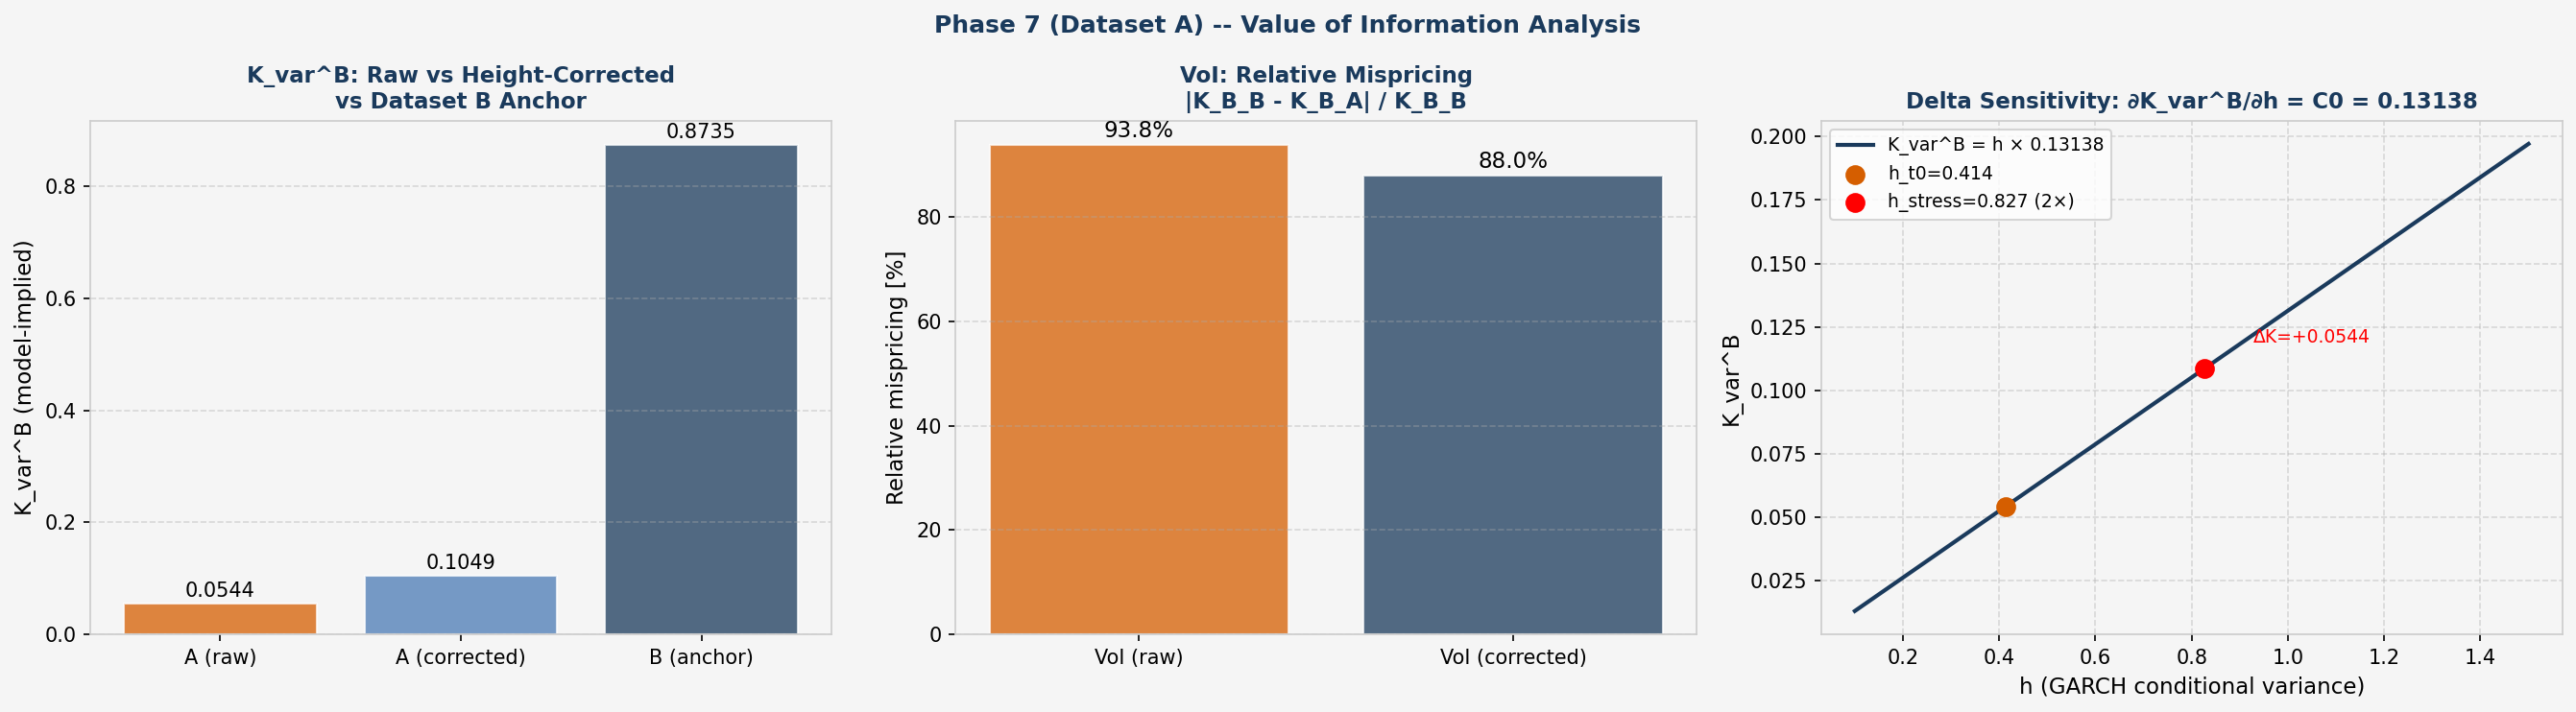
\includegraphics[width=\textwidth]{figures/phase7_A_voi_comparison.png}
\caption{Dataset A perspective}
\end{subfigure}
\hfill
\begin{subfigure}{0.48\textwidth}
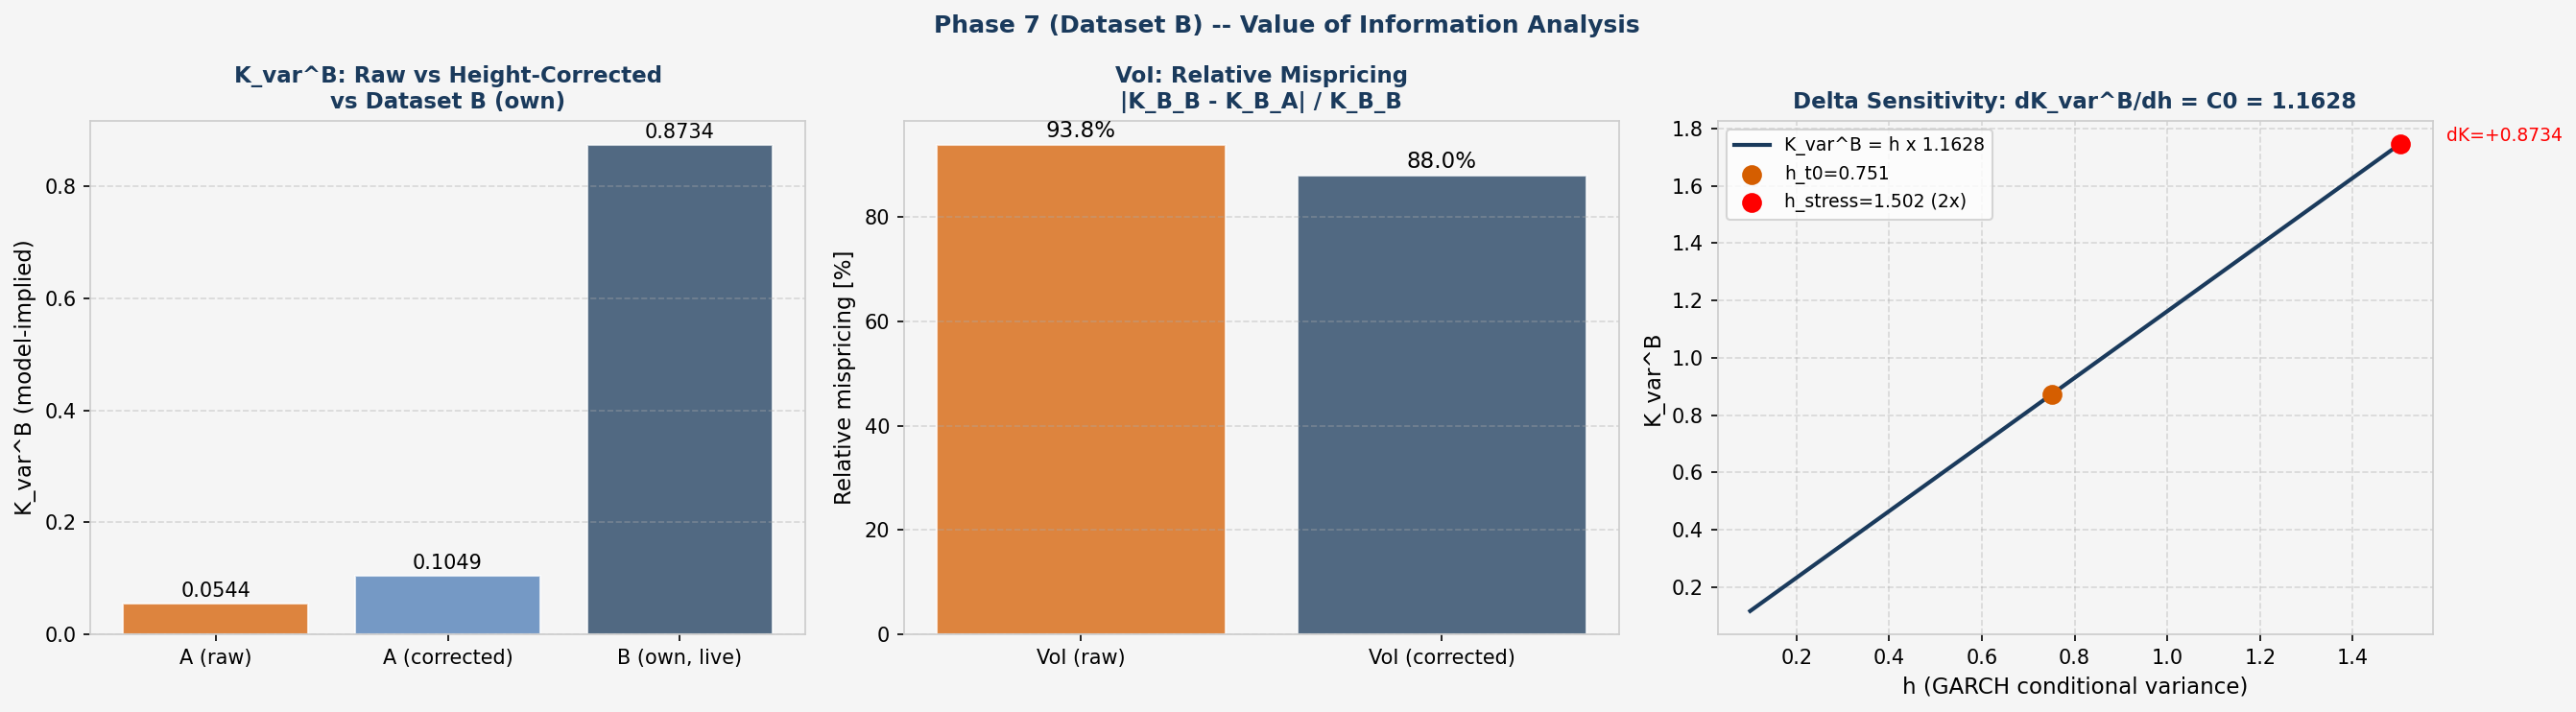
\includegraphics[width=\textwidth]{figures/phase7_B_voi_comparison.png}
\caption{Dataset B perspective}
\end{subfigure}
\caption{Value of Information analysis, computed from each dataset's own notebook. Each panel has three plots. \textbf{Left:} the model-implied fair strike as bars, for the raw Dataset~A value, its height-corrected counterpart, and the Dataset~B reference, showing how little of the gap the $1.9307\times$ correction of Equation~\eqref{eq:height} closes. \textbf{Centre:} the raw and height-corrected relative mispricing, 93.8\% and 88.0\%, as bars. \textbf{Right:} the delta sensitivity $K_{\text{var}}^B = h\,C_0$ plotted as a function of $h$, a straight line through the origin of slope $C_0$, with the pricing-date and stress values marked (Section~\ref{sec:delta}). The two panels differ only in which dataset's $C_0$ sets the slope in the right-hand plot; the left and centre plots report the same cross-dataset comparison from either side.}
\label{fig:voi}
\end{figure}

\subsection{The Empirical-Distance Metric}
\label{sec:voi-distance}

A second diagnostic was specified alongside the relative mispricing: the absolute distance between each dataset's unit-reconciled model strike and the market strike it is meant to approximate,
\begin{equation}
\mathrm{dist} = \bigl|K_{\text{var}}^A - K_{\text{var}}^{B,\text{scaled}}(h(t_0))\bigr|,
\end{equation}
with the ratio $\mathrm{dist}_A/\mathrm{dist}_B$ intended to measure how much closer to its own market the aligned model sits. The computed values are $113.918$ for Dataset~A, which is 99.93\% of that sample's Track~A level, and $113.024$ for Dataset~B, which is 99.89\% of its own, giving a ratio of $1.0079$.

The metric, as constructed, carries essentially no information, and the reason is the annualisation convention of Section~\ref{sec:reconciliation}: both scaled Track~B strikes are of order $0.1$ while both Track~A strikes are of order $113$, so each distance is, to within a tenth of a percent, just the Track~A level itself. A metric that returns the benchmark regardless of the model cannot discriminate between models. The Dataset~B notebook reaches the same verdict in its own output, observing that the $113$-unit gap ``swamps the smaller geographic/height effect this diagnostic was meant to isolate,'' and that assessment is endorsed here.

The rolling counterpart behaves the same way. The root mean squared distance between the rolling Track~A series and the rolling unit-reconciled Track~B series is $120.86$ for Dataset~A, computed over 1{,}335 overlapping days falling within 2016--2018, and $113.95$ for Dataset~B over 3{,}397 days spanning 2016--2024. Each sits within 6\% and 1\% respectively of its own Track~A level, and the difference between them reflects mainly the different and non-comparable evaluation windows rather than any property of the two models.

The conclusion is that the case for the aligned dataset does not rest, and cannot rest, on the distance between the model strike and the market strike, for two independent reasons: the distance metric as implemented is dominated by a units convention, and once the units are fully reconciled (Table~\ref{tab:reconciliation}) the proxy is if anything nearer the market level than the reference dataset is. The case rests instead on Section~\ref{sec:powercurve}. A model whose input explains 58.7\% of the variation in the series being hedged is usable for hedging; one whose input explains 0.01\% is not, whatever variance level it happens to imply. Dataset~A's apparent proximity to the market strike in reconciled units is a coincidence of level between two unrelated series, and is worth stating precisely because it is the sort of coincidence that a level-based validation metric would mistake for a successful calibration. This is the Value of Information properly understood: not that the proxy quotes the wrong number, but that it quotes a number carrying no information about the risk it would be used to transfer.

\subsection{Delta Sensitivity and the Stress Scenario}
\label{sec:delta}

Because the fair strike is linear in the conditional-variance state, its sensitivity is the seasonal constant itself,
\begin{equation}
\frac{\partial K_{\text{var}}^B}{\partial h} = C_0,
\end{equation}
equal to $0.13138$ for Dataset~A and $1.16277$ for Dataset~B. This is the variance swap's delta with respect to the volatility state, and it is constant: the instrument has no convexity in $h$, which follows directly from the piecewise-constant convention and is the pricing counterpart of the linearity of the payoff noted in Section~\ref{sec:varswap-def}.

A stress scenario in which a persistent wind regime shift doubles the conditional variance, $h_{\text{stress}} = 2h(t_0)$, shifts the strike by
\begin{equation}
\Delta K_{\text{var}}^B = (h_{\text{stress}} - h(t_0))\,C_0 = h(t_0)\,C_0 = K_{\text{var}}^B(h(t_0)),
\end{equation}
that is, by exactly the strike itself: $+0.0544$ for Dataset~A, taking the strike to $0.1087$, and $+0.8734$ for Dataset~B, taking it to $1.7467$. The identity is trivial but the risk-management reading is not. It says that the model-implied strike is proportional to the volatility state with no attenuation, so a hedging book marked on this model carries full linear exposure to a regime shift in $h$; and it says that the absolute size of that exposure is set by $C_0$, so the aligned dataset's book is $8.85$ times more sensitive in absolute terms than the proxy's, though identically sensitive in proportional terms. Whether such a doubling is plausible over a contract horizon is a question this framework can answer only indirectly: Section~2.3.1 puts the volatility half-life at 41.6 and 38.3 days, so a shock large enough to double $h$ would still retain roughly 70\% of its effect after 20 days and would not decay below a quarter of its initial size for about three months.

\subsection{Out-of-Time Validation}
\label{sec:oos}

Dataset~B's ten-year window permits a test that Dataset~A's four-year window does not. The full-sample unit-reconciled strike $K_{\text{var}}^{B,\text{scaled}}(h(t_0)) = 0.12075$ is held fixed as a model prediction and evaluated as a constant forecast of the rolling Track~A series, separately on the 1{,}570 days up to 31~December~2019 and the 1{,}827 days from 1~January~2020. The root mean squared errors are $113.232$ and $114.569$ respectively, an increase of 1.18\%.

The exercise must be read for exactly what it is. It is an out-of-time evaluation under fixed parameters, not genuine out-of-sample calibration: $C_0$ and $h(t_0)$ were both estimated on the full 2015--2024 window, so the hold-out period is contained in the estimation sample. It therefore tests whether the relationship the model captures is stable across the two halves of the decade, not whether the model would have forecast the second half from the first. And, for the reason given in Section~\ref{sec:voi-distance}, both root mean squared errors are dominated by the annualisation gap and are close to the Track~A level itself, so the 1.18\% deterioration is best read as a statement about the stability of Track~A across the two sub-periods rather than about the model. What it does establish, weakly but genuinely, is that nothing in the 2020--2024 window, including the price crisis and the substantial capacity additions of those years, destabilised the variance of generation log-returns enough to register.

\section{Risk Management: The CAWS Instrument}
\label{sec:caws}

\subsection{Definition and Fair Strike}
\label{sec:caws-def}

A variance swap is indifferent to the direction of the underlying's movement. It pays on realised variance, so a sustained calm period, the single event a wind producer most needs protection against, registers as low variance rather than as a loss. The left tail of wind-linked revenue risk is therefore not addressed by the instrument of Section~\ref{sec:varswap}, and this section evaluates a complement to it.

The Cumulative Accumulated Wind Speed index of \citet{AlexandridisZapranis2013} is taken in the normalised rolling-annual-mean form defined in Equation~(1.1) of Section~1.4.4,
\begin{equation}
\mathrm{CAWS}_t = \frac{1}{252}\sum_{s=t-252}^{t} W(s),
\end{equation}
with $W(s)$ the daily mean wind speed in m/s. Normalising by the window length rather than accumulating raw sums keeps the index in m/s and therefore comparable across the two measurement heights. The strike is the full-sample mean, $K_{\mathrm{CAWS}} = \mathbb{E}[\mathrm{CAWS}_t]$, and a producer buying the instrument at that strike receives
\begin{equation}
\Pi_t = N \times (K_{\mathrm{CAWS}} - \mathrm{CAWS}_t),
\end{equation}
which is positive when realised wind falls short of the strike. The instrument is thus a put on the wind resource: it pays in exactly the state, a calm year, in which the producer's generation revenue is depressed.

The fitted strikes are $K_{\mathrm{CAWS}} = 2.4644$~m/s for Dataset~A, computed over 1{,}263 rolling observations with a rolling standard deviation of $0.2013$~m/s, and $8.0531$~m/s for Dataset~B, over 3{,}454 rolling observations with a rolling standard deviation of $0.5002$~m/s. Both are consistent with the raw sample means of Tables~1.1 and~1.2, as they must be.

\subsection{Distribution Metrics on Non-Overlapping Annual Observations}
\label{sec:caws-metrics}

The rolling construction induces severe serial correlation: adjacent values of $\mathrm{CAWS}_t$ share 251 of their 252 constituent observations and are therefore almost perfectly correlated, so any standard deviation or quantile computed on the rolling series would be badly biased. All distribution metrics are consequently computed on non-overlapping calendar-year means, one independent observation per year, giving four observations for Dataset~A and ten for Dataset~B. The rolling series is retained only for plotting. Table~\ref{tab:caws-annual} reports the annual observations and Table~\ref{tab:caws-metrics} the resulting metrics.

\begin{table}[htbp]
\centering
\caption{Non-overlapping annual CAWS observations and payoffs, both datasets.}
\label{tab:caws-annual}
\begin{tabular}{l r r r r}
\toprule
& \multicolumn{2}{c}{\textbf{Dataset A} ($K = 2.4644$)} & \multicolumn{2}{c}{\textbf{Dataset B} ($K = 8.0531$)} \\
\textbf{Year} & \textbf{CAWS [m/s]} & \textbf{Payoff} & \textbf{CAWS [m/s]} & \textbf{Payoff} \\
\midrule
2015 & $2.4872$ & $-0.0228$ & $8.5626$ & $-0.5095$ \\
2016 & $2.5041$ & $-0.0397$ & $7.7162$ & $+0.3369$ \\
2017 & $2.2993$ & $+0.1650$ & $8.0879$ & $-0.0347$ \\
2018 & $2.5853$ & $-0.1209$ & $7.8396$ & $+0.2135$ \\
2019 & --- & --- & $8.2526$ & $-0.1995$ \\
2020 & --- & --- & $8.2830$ & $-0.2299$ \\
2021 & --- & --- & $7.6513$ & $+0.4018$ \\
2022 & --- & --- & $8.1063$ & $-0.0532$ \\
2023 & --- & --- & $8.1416$ & $-0.0885$ \\
2024 & --- & --- & $8.0410$ & $+0.0121$ \\
\bottomrule
\end{tabular}
\end{table}

\begin{table}[htbp]
\centering
\caption{CAWS distribution metrics on non-overlapping annual observations.}
\label{tab:caws-metrics}
\begin{tabular}{l r r}
\toprule
\textbf{Metric} & \textbf{Dataset A} & \textbf{Dataset B} \\
\midrule
$K_{\mathrm{CAWS}}$ [m/s] & $2.4644$ & $8.0531$ \\
Annual observations $n$ & $4$ & $10$ \\
Mean payoff [m/s] & $-0.0046$ & $-0.0151$ \\
Std.\ deviation of payoff [m/s] & $0.1209$ & $0.2754$ \\
Sharpe ratio & $-0.0379$ & $-0.0549$ \\
$\mathrm{VaR}_{5\%}$ [m/s] & $-0.1087$ & $-0.3837$ \\
$\mathrm{CVaR}_{5\%}$ [m/s] & $-0.1209$ & $-0.5095$ \\
\midrule
$\mathrm{CVaR}_{5\%}$ as \% of $K_{\mathrm{CAWS}}$ & $-4.91\%$ & $-6.33\%$ \\
Largest positive payoff [m/s] & $+0.1650$ (2017) & $+0.4018$ (2021) \\
\quad as \% of $K_{\mathrm{CAWS}}$ & $6.70\%$ & $4.99\%$ \\
\bottomrule
\end{tabular}
\end{table}

\subsection{Reading the Tail}
\label{sec:caws-tail}

Three properties of Table~\ref{tab:caws-metrics} determine how it should be read, and each cuts against a reading offered in the source documents.

First, the mean payoff is near zero by construction, because the strike is set to the sample mean of the very series it is evaluated against. It is $-0.0046$ and $-0.0151$~m/s, differing from exactly zero only because the strike is the mean of the rolling series while the payoffs are computed on calendar-year means. The Sharpe ratios of $-0.038$ and $-0.055$ that follow from dividing a near-zero mean by a positive standard deviation are therefore not measures of the instrument's performance; they carry no information beyond the arithmetic that produced them, and the Dataset~A notebook says as much in its own output. A Sharpe ratio is a meaningful statistic for a traded position with a market-determined entry price; it is not one for a contract struck at the mean of its own underlying.

Second, and more consequentially, the sign convention means that the reported $\mathrm{CVaR}_{5\%}$ describes the wrong tail for a hedger. The payoff is $K_{\mathrm{CAWS}} - \mathrm{CAWS}$, so a negative payoff arises in a \emph{windy} year. Dataset~B's $\mathrm{CVaR}_{5\%} = -0.5095$~m/s is the payoff of 2015, the windiest year of the decade at $8.5626$~m/s, in which the producer's own generation was at its highest. That is not a risk; it is the hedge behaving as designed, with the producer paying the insurance leg out of an unusually good year's revenue. The Dataset~B phase document reads this figure as a downside, describing it as ``a worst-case scenario (5\% tail risk) of wind being 0.5 m/s below fair strike'' implying an 18\% revenue loss, which inverts the sign of the observation: 2015 was 0.51~m/s \emph{above} strike, not below. The tail that matters to a producer is the opposite one, the largest positive payoffs, and those are reported in the final rows of Table~\ref{tab:caws-metrics}.

Third, with $n = 4$ and $n = 10$ the $\mathrm{CVaR}_{5\%}$ is not a tail average at all. In both datasets it equals the single most negative annual observation exactly, because no observation other than the minimum falls at or below the fifth percentile of so small a sample. The two conditional value-at-risk figures are therefore sample minima under another name, and the same holds for the fifth-percentile value-at-risk, which is an interpolation between the two most negative points. This is the unavoidable cost of the non-overlapping-window choice made in Section~\ref{sec:caws-metrics}: it purchases freedom from serial-correlation bias at the price of four and ten observations respectively, and the resulting tail statistics are descriptive rather than inferential, exactly as Section~1.2 anticipated.

With those three corrections applied, what the table shows is the following. The protection leg of the instrument is economically substantial. The calmest year in Dataset~B's decade, 2021, came in 4.99\% below the strike and would have paid $+0.4018$~m/s per unit of notional; Dataset~A's calmest year, 2017, came in 6.70\% below and would have paid $+0.1650$~m/s. Translated through the cubic power relation of Section~\ref{sec:powercurve}, a 4.99\% shortfall in mean wind speed corresponds to roughly a 14\% shortfall in generation, and a 6.70\% shortfall to roughly 19\%. Applied to the illustrative 100~MW farm of Section~1.1, generating some 225{,}100~MWh in a normal year, a 14\% shortfall is about 32{,}000~MWh; valued at the full-sample mean day-ahead price of \texteuro{}71.38/MWh, that is roughly \texteuro{}2.3 million of foregone gross revenue in a single calm year, or about \texteuro{}1.1 million at the 2015--2020 mean price and \texteuro{}4.1 million at the 2021--2024 mean. These are order-of-magnitude illustrations built transparently from a stated capacity factor and observed prices, in the manner of Section~1.1, and the cubic mapping is a first-order approximation that ignores the difference between the cube of the mean and the mean of the cube.

A single episode in the data is worth noting alongside them, with its limits stated. Dataset~B's calmest year, 2021, coincided with the onset of the European energy-price crisis, so a producer suffering that volumetric shortfall would in fact have sold the reduced output into a sharply higher price and might well have earned more, not less, than in a normal year. That is the natural hedge of Section~\ref{sec:merit} operating at its most favourable. It should not be generalised: the 2021--2022 price surge was driven by gas markets rather than by German wind conditions, and a single coincidence of that kind is not evidence that the natural hedge places a floor under the volumetric downside. If anything it illustrates the asymmetry stated in Section~1.1, since the same producer would have received no comparable compensation in the calm years of a normal price regime.

Finally, the cross-dataset comparison of the CAWS metrics needs the same units discipline applied to the variance swap in Section~\ref{sec:reconciliation}. Dataset~B's $\mathrm{CVaR}_{5\%}$ is $4.21$ times Dataset~A's in m/s, and the Dataset~B phase document reads this as ``higher tail risk (4.2$\times$).'' It is not: it is chiefly the ratio of the two mean wind speeds, since a metric denominated in m/s at 100~m cannot be compared with one at 10~m. Normalised by the respective strikes, the two figures are $-4.91\%$ and $-6.33\%$, a difference of about 30\% rather than of a factor of four. The genuine advantage of Dataset~B here is not a larger tail but a better-estimated one: ten independent annual observations against four.

\begin{figure}[htbp]
\centering
\begin{subfigure}{0.48\textwidth}
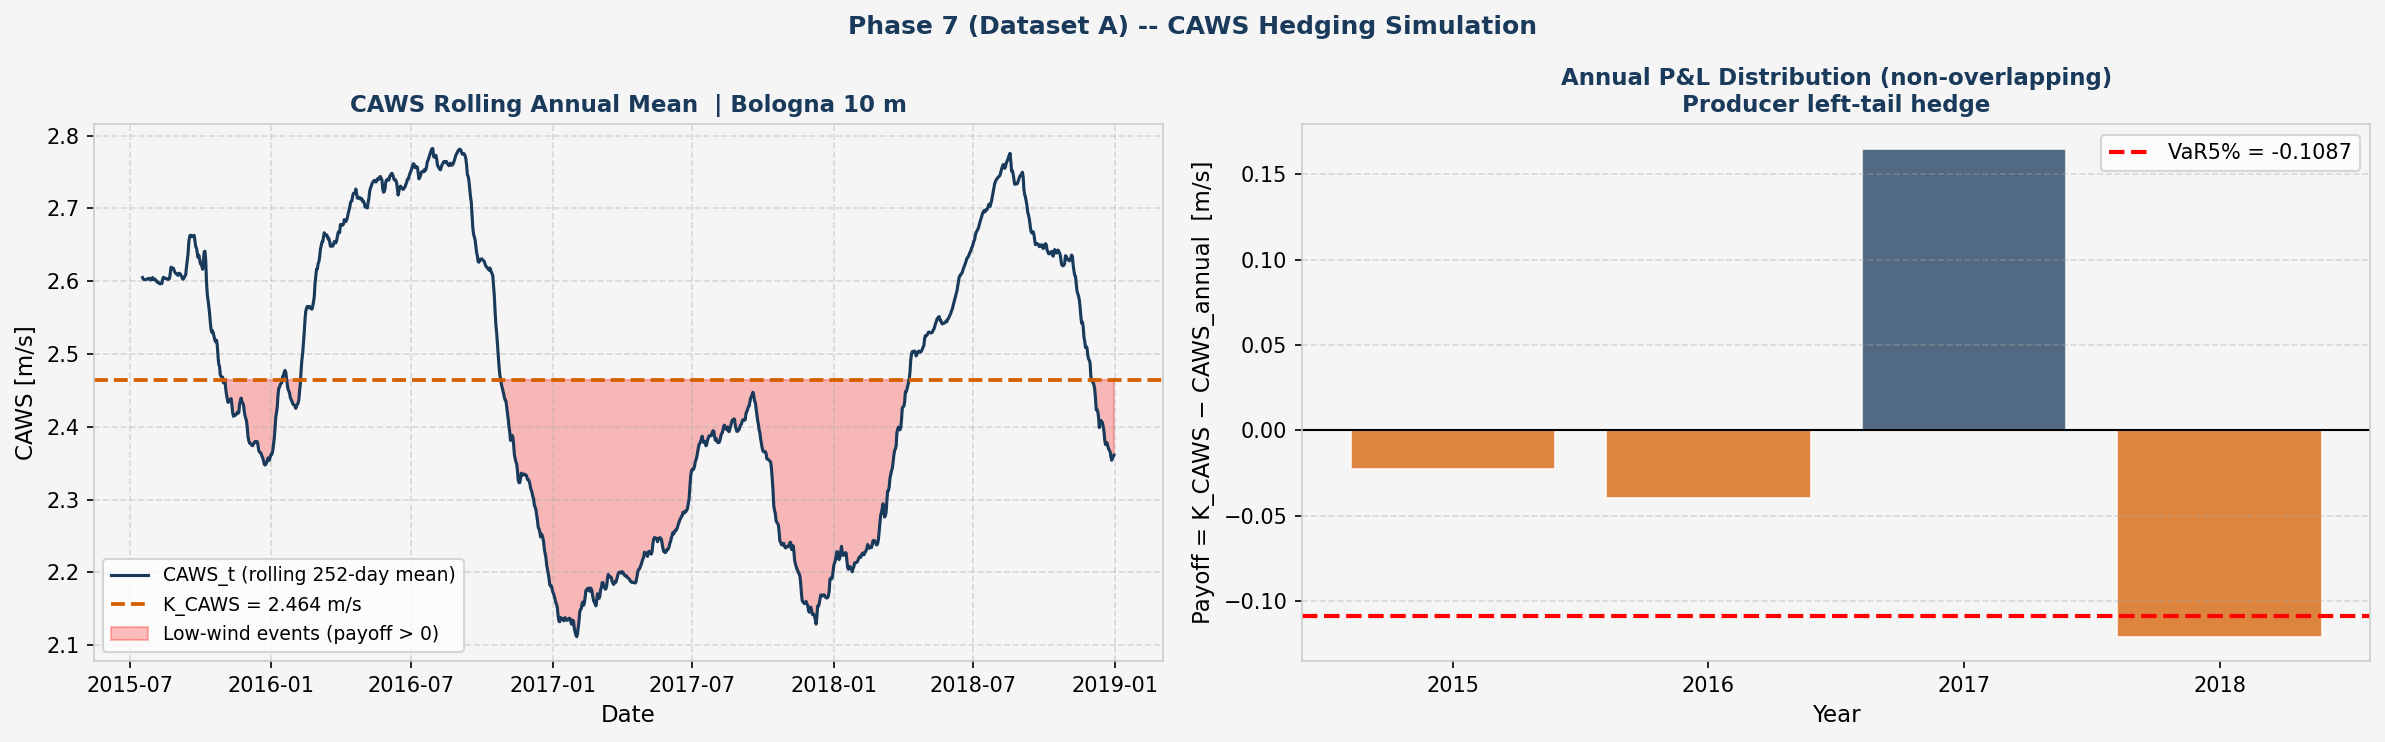
\includegraphics[width=\textwidth]{figures/phase7_A_caws_hedge_pnl.png}
\caption{Dataset A}
\end{subfigure}
\hfill
\begin{subfigure}{0.48\textwidth}
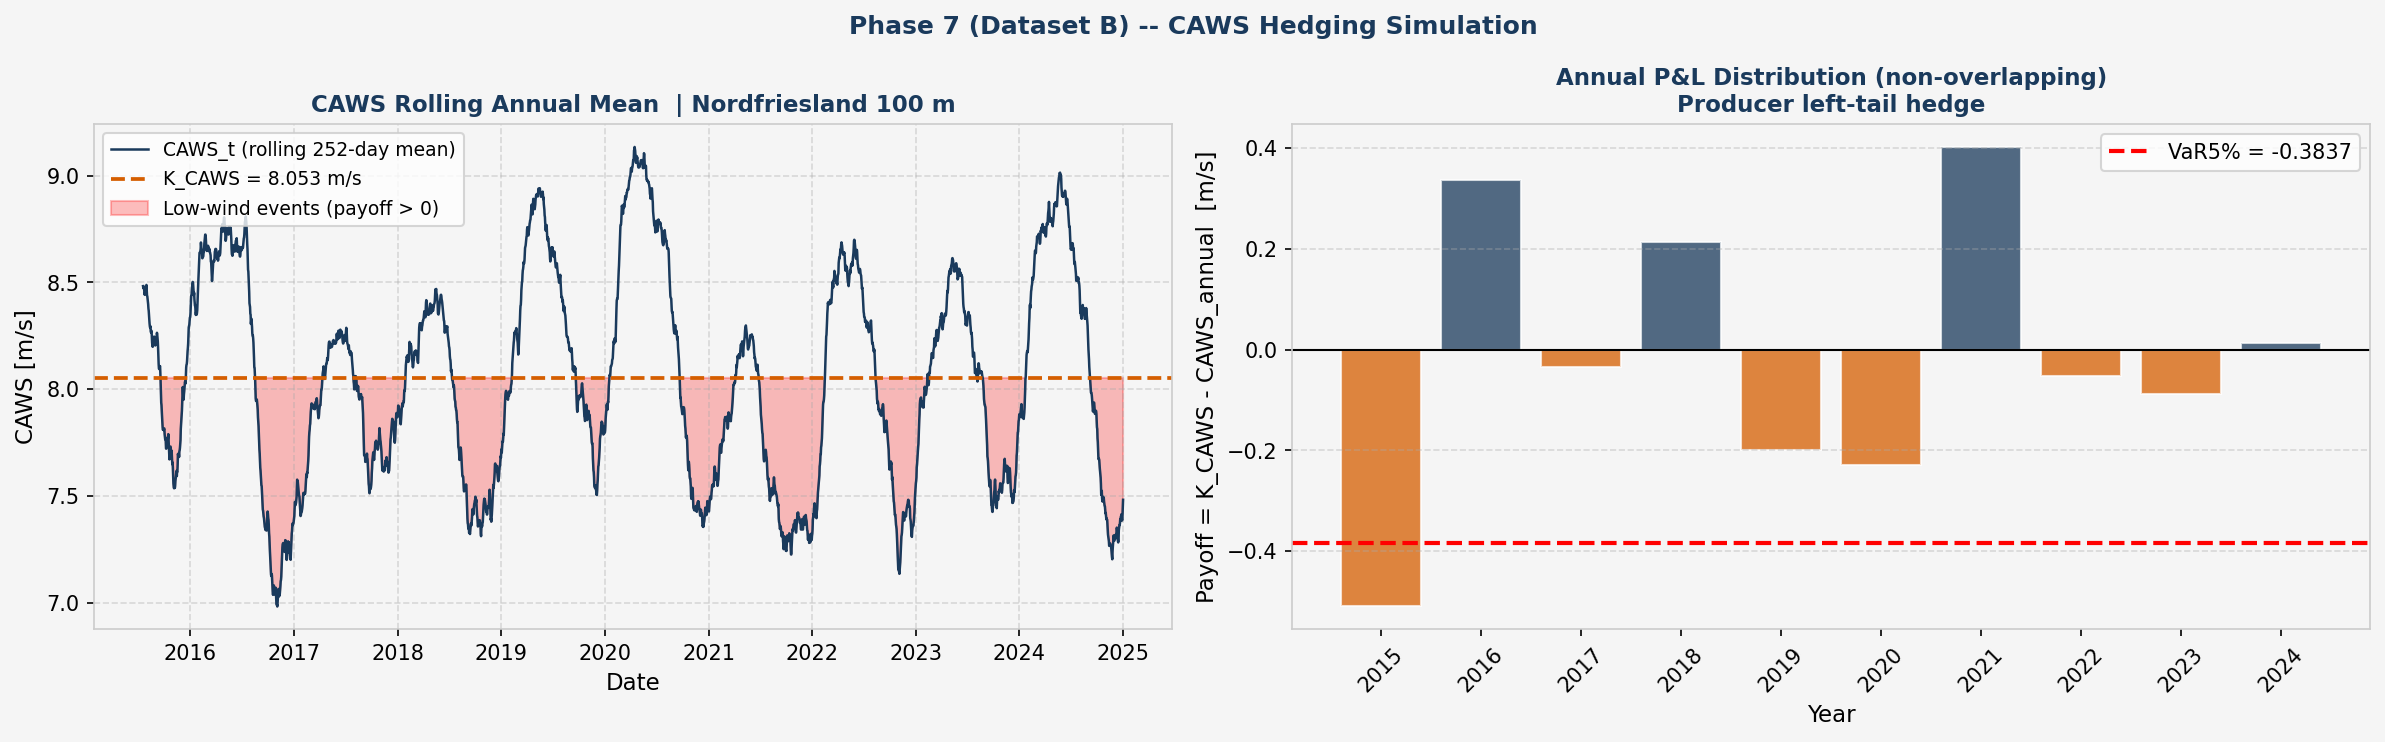
\includegraphics[width=\textwidth]{figures/phase7_B_caws_hedge_pnl.png}
\caption{Dataset B}
\end{subfigure}
\caption{CAWS hedging simulation, both datasets. Each panel has two plots. \textbf{Left:} the rolling 252-day CAWS series in m/s with the fair strike $K_{\mathrm{CAWS}}$ marked as a horizontal line; the smoothness of the series is the serial correlation that motivates computing all metrics on non-overlapping annual observations instead. \textbf{Right:} the non-overlapping annual payoffs $K_{\mathrm{CAWS}} - \mathrm{CAWS}_y$ as bars, one per calendar year, with the zero line and the fifth-percentile value-at-risk marked. Positive bars are the protection leg, paying in calm years; negative bars are the premium leg, paid in windy years. Note that the two panels use different vertical scales, in m/s at 10~m and at 100~m respectively, and should be compared only after the normalisation of Table~\ref{tab:caws-metrics}.}
\label{fig:caws}
\end{figure}

\section{Conclusions}
\label{sec:conclusions}

\subsection{Summary of Findings}
\label{sec:concl-summary}

Table~\ref{tab:summary} collects the chapter's principal results. The three research questions posed in Section~1.2 can now be answered.

\begin{table}[htbp]
\centering
\small
\caption{Summary of Chapter 3 results, both datasets.}
\label{tab:summary}
\begin{tabularx}{\textwidth}{>{\raggedright\arraybackslash}p{0.28\textwidth} >{\raggedright\arraybackslash}X >{\raggedright\arraybackslash}X}
\toprule
& \textbf{Dataset A (Bologna 10~m)} & \textbf{Dataset B (Nordfriesland 100~m)} \\
\midrule
Track A fair strike $K_{\text{var}}^A$ & $113.999$ & $113.145$ \\
Track B fair strike $K_{\text{var}}^B(h(t_0))$ & $0.05435$ & $0.87336$ \\
Track B, unit-reconciled (Table~\ref{tab:reconciliation}) & $132.9$ & $328.8$ \\
Power curve $R^2$ & $0.0001$ ($p = 0.723$) & $0.5871$ ($p < 0.001$) \\
Merit-order $\rho(G,P)$ & \multicolumn{2}{c}{$-0.162$ full sample; $-0.476$ pre-2018-10, $-0.275$ post} \\
AR(4) RMSE vs.\ persistence & $0.7802$ vs.\ $0.8868$ ($12.0\%$) & $0.8681$ vs.\ $1.0046$ ($13.6\%$) \\
Diebold--Mariano statistic & $8.265$ ($p < 10^{-15}$) & $16.758$ ($p < 10^{-16}$) \\
GARCH adequacy & All tests pass & Rejects at $z^2$ lag 5 and ARCH-LM \\
Jarque--Bera, AR(4) errors & $108.87$ ($p < 0.001$) & $17.05$ ($p < 0.001$) \\
Value of Information (raw / corrected) & \multicolumn{2}{c}{$93.8\%$ / $88.0\%$, Dataset B as reference} \\
$K_{\mathrm{CAWS}}$ & $2.4644$~m/s ($n = 4$) & $8.0531$~m/s ($n = 10$) \\
$\mathrm{CVaR}_{5\%}$, \% of strike & $-4.91\%$ & $-6.33\%$ \\
\bottomrule
\end{tabularx}
\end{table}

\paragraph{RQ1: can the framework price the instrument?} Yes, and in closed form. Under the $\theta = 0$ benchmark the fair strike collapses to $K_{\text{var}}^B = h \times C_0$, requiring no numerical integration and no Girsanov computation, and Section~\ref{sec:trackb} evaluates it at four volatility states for both datasets. Two qualifications attach to that affirmative answer. The strike is a conditional quantity that inherits the pricing date's volatility state, and for Dataset~A that dependence is material, spanning a factor of $2.42$ across the four scenarios. And the instrument's tractability comes from freezing $h$: the model has no convexity in the volatility state, so it prices a variance swap but would not price an option on variance, for which the \citet{Heston1993} characteristic function of Section~2.5.5 would have to be evaluated rather than merely written down.

\paragraph{RQ2: what is the Value of Information?} Pricing the identical model on the proxy rather than the aligned dataset understates the fair strike by 93.8\%, falling to 88.0\% once measurement height is corrected. The height correction closes little of the gap, and no plausible profile exponent would close it, so the residual is not a height effect. It decomposes into a factor of $8.85$ in the seasonal-variance constant $C_0$ and $1.82$ in the GARCH state, locating the discrepancy in the site rather than in the volatility regime.

The more careful answer, developed in Sections~\ref{sec:reconciliation} and~\ref{sec:voi-distance}, is that these figures measure the right thing for the wrong reason. Once both strikes are mapped onto the common axis of generation log-return variance, the $16.07\times$ ratio falls to about $2.5\times$, and the purely climatological part of it to about $1.36\times$: the two sites have nearly identical coefficients of variation, $0.384$ and $0.401$, and on the relative scale the instrument actually references they are close to equivalent. What separates them is not the level of variance they imply but whether that variance has anything to do with the quantity being hedged. Nordfriesland hub-height wind explains 58.7\% of the daily variation in the generation series; Bologna 10~m wind explains 0.01\%, with a slope not distinguishable from zero. The Value of Information is properly located there. A proxy that quotes a coincidentally reasonable number while carrying no information about the risk being transferred is more dangerous than one that quotes an obviously wrong number, because only the second announces itself.

\paragraph{RQ3: how effective is CAWS as a left-tail hedge?} The instrument does what it is designed to do. Its payoff is positive in precisely the calm years that depress generation revenue, and the magnitudes are economically material: the calmest year in Dataset~B's decade would have paid $+0.4018$~m/s per unit of notional against a shortfall of roughly 14\% in generation, worth on the order of \texteuro{}2.3 million of gross revenue on the illustrative 100~MW farm. The risk metrics reported for it, however, require the three corrections of Section~\ref{sec:caws-tail}: the Sharpe ratio is uninformative because the strike is the mean of its own underlying, the conditional value-at-risk describes the premium leg rather than the protection leg, and with four and ten annual observations it is a sample minimum rather than a tail average. Read correctly, the cross-dataset comparison shows not that Dataset~B carries four times the tail risk but that it estimates a similar relative tail from two and a half times as many independent observations.

\paragraph{On the model hierarchy.} A fourth result cuts across all three questions. Every fitted specification beats persistence decisively, and all four are observationally equivalent to one another at a one-day horizon, by construction rather than by coincidence. Point-forecast accuracy therefore cannot discriminate among them, which is precisely why this thesis evaluates them on pricing and hedging criteria instead. The GARCH layer earns its place by supplying $h$, the state variable that carries the entire conditional content of the fair strike; the CAR(4) embedding of \citet{BenthSaltyteBenth2009} earns its place by permitting pricing at maturities off the daily grid; and the NIG extension, on the evidence of Section~\ref{sec:forecast-dist} and Section~2.4.4, earns rather little in either dataset and is retained as a documented robustness extension rather than as the operative model.

\subsection{Limitations}
\label{sec:concl-limits}

Five limitations bound what has been established, and they are stated in descending order of how much they constrain the conclusions.

\paragraph{The $\theta = 0$ benchmark.} The pricing measure is not identified by the data. No liquid options market exists on German wind speed or on the SMARD generation aggregate, and the only traded wind derivatives reference Norwegian wind, so the market price of risk cannot be calibrated and is set to zero as a tractable benchmark (Section~2.5.4). Every strike in this chapter is therefore a physical-measure expectation. The evidence from temperature markets reviewed in Section~1.3.6, where \citet{HardleLopezCabrera2009} and \citet{DorfleitnerWimmer2010} both recover a market price of weather risk significantly different from zero, suggests a true market-implied strike would lie above it, since producers seeking protection would be expected to pay a premium over the physical expectation. The direction is a hypothesis and the magnitude is unknown.

\paragraph{Commensurability of the cross-dataset comparison.} The headline Value of Information figures compare two variances expressed in two different Box--Cox measurement scales, and Section~\ref{sec:reconciliation} shows that a substantial part of the $16.07\times$ gap is attributable to that difference and to the six-year separation of the two pricing dates rather than to the sites. The figures accurately describe what the two calibrated pipelines quote and are retained on that basis, but they should not be read as a scale-free measure of climatological difference.

\paragraph{Spatial aggregation.} Both models are calibrated on a single grid point while the hedged quantity is a national fleet aggregate. Spatial averaging removes variance, which is the most likely explanation for both models overstating the market strike by factors of three to four in reconciled units, and it also caps the achievable power-curve $R^2$ well below one. A multi-site or spatially averaged wind input would address this and would be the natural first extension of the pricing exercise.

\paragraph{Daily frequency.} The stochastic-volatility parameters $(\kappa_V, \bar v, \xi, \rho)$ are not identified at daily frequency, for the reasons set out in Section~2.5.7, and the CIR proxies used in Chapter~2 are moment-matched from the GARCH fit rather than estimated. The same coarseness shows in the Dataset~B diagnostics of Section~\ref{sec:garch-diag}, where short-lag volatility structure survives a single-component GARCH filter.

\paragraph{Sample size for tail statistics.} The non-overlapping-window choice that makes the CAWS risk metrics unbiased also reduces them to four and ten observations. The resulting tail statistics are descriptive, and the cross-dataset comparison of Section~\ref{sec:caws-tail} rests on the sign and relative dispersion of the payoff rather than on a fifth-percentile quantile estimated from four points.

\subsection{Future Work}
\label{sec:concl-future}

Three extensions follow directly from those limitations, and one from the results themselves.

The first is option-implied calibration of $\theta$. EEX German power options are the most liquid in Europe, and extracting a wind risk premium from them is the designated route to replacing the $\theta = 0$ benchmark with an estimated pricing measure. The obstacle is that those options are written on the power price rather than on wind speed or generation, so the exercise requires a joint model of price and generation capable of separating the wind premium from the power-price premium; it is a substantially larger undertaking than a straightforward calibration, and the \citet{CarrLee2009} replication framework would supply the theoretical scaffolding for it.

The second is estimation at higher frequency. Hourly ERA5 reanalysis at the same coordinates would raise the observation count by roughly two orders of magnitude, resolve the intraday volatility clustering and diurnal boundary-layer cycles that daily aggregation smooths away, and make $\xi$ separately identifiable from $\kappa_V$. That would convert Chapter~2's stochastic-volatility framework from a theoretical embedding into an estimated model, and would permit pricing instruments, such as options on variance, that the piecewise-constant convention cannot reach.

The third is a spatially aggregated wind input, replacing the single grid point with a capacity-weighted average across the German onshore fleet. This addresses the variance overstatement identified in Section~\ref{sec:reconciliation} directly, and would be expected to raise the power-curve $R^2$ above the 0.587 achieved from Nordfriesland alone.

A fourth extension is suggested by the results rather than by their limitations. The finding of Section~\ref{sec:voi-distance}, that a wholly uninformative proxy can nonetheless imply a variance level close to the market's, argues for evaluating candidate datasets on explanatory power for the hedged quantity before, and not after, comparing the strikes they imply. A systematic screening of candidate reanalysis grid points on power-curve $R^2$, prior to any pricing, would be a cheap and general-purpose diagnostic for this class of problem.

\subsection{Implications for Producers and Risk Managers}
\label{sec:concl-implications}

Three practical conclusions follow for a German onshore wind producer or the risk manager of a renewables-heavy portfolio.

The natural hedge afforded by the merit-order effect is real but weak and asymmetric. At $\rho = -0.162$ over the full sample, and $-0.476$ and $-0.275$ within the two price regimes, high wind does depress the price a producer captures, dampening revenue variance relative to the independent case. But it erodes the upside without placing a floor under the downside, and the residual volumetric exposure it leaves is what a wind-linked instrument is for.

The two instruments priced here are complements, not substitutes, and address different risks. The variance swap transfers the volatility of generation, and its fair strike, at an annualised realised variance near 114 with a year-to-year range from 95 to 132, is both large and genuinely variable. The CAWS instrument transfers the level of the wind resource, paying in the calm years to which the variance swap is by construction indifferent. A producer concerned primarily with the revenue consequences of a wind drought needs the second; one concerned with cash-flow predictability needs the first.

Data alignment is not a refinement to be added once the model works; it is a precondition for the model meaning anything. This is the chapter's central practical message and the one it would most want a practitioner to take away. A model calibrated on a misaligned proxy produced, in this exercise, a fair strike that was 93.8\% below the aligned one on the model's own scale and yet, on a fully reconciled scale, sat closer to the observed market level than the aligned model did. Neither comparison would have revealed the problem. Only regressing the candidate wind series on the quantity actually being hedged did, returning $R^2 = 0.0001$ against $0.5871$. Before a wind derivative is priced, the wind series it is priced from should be required to explain the cash flows it is meant to hedge.

\newpage
\begin{thebibliography}{99}

\bibitem[Alexandridis and Zapranis(2013)]{AlexandridisZapranis2013}
Alexandridis, A., \& Zapranis, A. (2013).
Wind derivatives: modeling and pricing.
\textit{Computational Economics}, 41(3), 299--326.

\bibitem[Barndorff-Nielsen and Shephard(2001)]{BarndorffNielsenShephard2001}
Barndorff-Nielsen, O. E., \& Shephard, N. (2001).
Non-Gaussian Ornstein--Uhlenbeck-based models and some of their uses in financial economics.
\textit{Journal of the Royal Statistical Society: Series B}, 63(2), 167--241.

\bibitem[Benth and \v{S}alty\.{t}\.{e} Benth(2009)]{BenthSaltyteBenth2009}
Benth, F. E., \& \v{S}alty\.{t}\.{e} Benth, J. (2009).
Dynamic pricing of wind futures.
\textit{Energy Economics}, 31(1), 16--24.

\bibitem[Bollerslev(1986)]{Bollerslev1986}
Bollerslev, T. (1986).
Generalized autoregressive conditional heteroskedasticity.
\textit{Journal of Econometrics}, 31(3), 307--327.

\bibitem[Carr and Lee(2009)]{CarrLee2009}
Carr, P., \& Lee, R. (2009).
Volatility derivatives.
\textit{Annual Review of Financial Economics}, 1, 1--21.

\bibitem[Diebold and Mariano(1995)]{DieboldMariano1995}
Diebold, F. X., \& Mariano, R. S. (1995).
Comparing predictive accuracy.
\textit{Journal of Business \& Economic Statistics}, 13(3), 253--263.

\bibitem[Dorfleitner and Wimmer(2010)]{DorfleitnerWimmer2010}
Dorfleitner, G., \& Wimmer, M. (2010).
The pricing of temperature futures at the Chicago Mercantile Exchange.
\textit{Journal of Banking \& Finance}, 34(6), 1360--1370.

\bibitem[Engle(1982)]{Engle1982}
Engle, R. F. (1982).
Autoregressive conditional heteroscedasticity with estimates of the variance of United Kingdom inflation.
\textit{Econometrica}, 50(4), 987--1007.

\bibitem[H\"ardle and L\'opez Cabrera(2009)]{HardleLopezCabrera2009}
H\"ardle, W. K., \& L\'opez Cabrera, B. (2009).
\textit{Implied market price of weather risk} (SFB 649 Discussion Paper No.\ 2009-001).
Humboldt-Universit\"at zu Berlin, Collaborative Research Center 649 ``Economic Risk.''

\bibitem[Harvey et al.(1997)Harvey, Leybourne, and Newbold]{HarveyEtAl1997}
Harvey, D., Leybourne, S., \& Newbold, P. (1997).
Testing the equality of prediction mean squared errors.
\textit{International Journal of Forecasting}, 13(2), 281--291.

\bibitem[Heston(1993)]{Heston1993}
Heston, S. L. (1993).
A closed-form solution for options with stochastic volatility with applications to bond and currency options.
\textit{Review of Financial Studies}, 6(2), 327--343.

\bibitem[Peterson and Hennessey(1978)]{PetersonHennessey1978}
Peterson, E. W., \& Hennessey, J. P., Jr. (1978).
On the use of power laws for estimates of wind power potential.
\textit{Journal of Applied Meteorology}, 17(3), 390--394.

\bibitem[Tol(1997)]{Tol1997}
Tol, R. S. J. (1997).
Autoregressive conditional heteroscedasticity in daily wind speed measurements.
\textit{Theoretical and Applied Climatology}, 56(1--2), 113--122.

\end{thebibliography}

\end{document}
